% \documentclass[oneside,12pt]{report} % ,twoside,draft,openright] % report e' per la tesi
\documentclass[11pt]{article}

\usepackage{setspace,graphicx,epstopdf,amsmath,amsfonts,amssymb,amsthm} %,versionPO}
\usepackage{marginnote,datetime,enumitem,subfigure,rotating,fancyvrb}
\usepackage{hyperref,float} % commenta se vuoi eiminare i link delle ref, vd sotto
\usepackage[longnamesfirst]{natbib}
\usdate

% hyperlink setup
\hypersetup{
	colorlinks=true,       % false: boxed links; true: colored links
	linkcolor=red,          % color of internal links (change box color with linkbordercolor)
	citecolor=green,        % color of links to bibliography
	filecolor=magenta,      % color of file links
	urlcolor=cyan           % color of external links
%, 	hidelinks		        % hide links (removing color and border)
}

% Save original definition of \marginpar
\let\oldmarginpar\marginpar

% Workaround for todonotes problem with natbib (To Do list title comes out wrong)
\makeatletter\let\chapter\@undefined\makeatother % Undefine \chapter for todonotes

% Define note commands
\newcommand{\smalltodo}[2][] {\todo[caption={#2}, size=\scriptsize, fancyline, #1] {\begin{spacing}{.5}#2\end{spacing}}}
\newcommand{\rhs}[2][]{\smalltodo[color=green!30,#1]{{\bf RS:} #2}}
\newcommand{\rhsnolist}[2][]{\smalltodo[nolist,color=green!30,#1]{{\bf RS:} #2}}
\newcommand{\rhsfn}[2][]{%  To be used in footnotes (and in floats)
\renewcommand{\marginpar}{\marginnote}%
\smalltodo[color=green!30,#1]{{\bf RS:} #2}%
\renewcommand{\marginpar}{\oldmarginpar}}
%\newcommand{\textnote}[1]{\ifnotes{{\noindent\color{red}#1}}{}}
\newcommand{\textnote}[1]{\ifnotes{{\colorbox{yellow}{{\color{red}#1}}}}{}}

% Command to start a new page, starting on odd-numbered page if twoside option 
% is selected above
\newcommand{\clearRHS}{\clearpage\thispagestyle{empty}\cleardoublepage\thispagestyle{plain}}

% Number paragraphs and subparagraphs and include them in TOC
\setcounter{tocdepth}{2}

% Nel caso non voglia alcun indentation con un nuovo paragrafo 
% \setlength{\parindent}{0pt}

% JFE-specific includes:
\usepackage{indentfirst} % Indent first sentence of a new section.
%\usepackage{jfe}          

% JFE-specific formatting of sections, etc.
% Theorems and the like
\newtheorem{theorem}{Theorem}[section]
\newtheorem{assumption}{Assumption}[section]
\newtheorem{proposition}{Proposition}
\newtheorem{conjecture}{Conjecture}
\newtheorem{lemma}{Lemma}[section]
\newtheorem{corollary}{Corollary}
\newtheorem{condition}{Condition}

%%%%%%%%%%%%%%%%%%%%%%%%%%%%%
%%%  to insert Python code: use 'listings' package
\usepackage{color}
\usepackage{listings}

\definecolor{Code}{rgb}{0,0,0}
\definecolor{Decorators}{rgb}{0.5,0.5,0.5}
\definecolor{Numbers}{rgb}{0.5,0,0}
\definecolor{MatchingBrackets}{rgb}{0.25,0.5,0.5}
\definecolor{Keywords}{rgb}{0,0,1}
\definecolor{self}{rgb}{0,0,0}
\definecolor{Strings}{rgb}{0,0.63,0}
\definecolor{Comments}{rgb}{0,0.63,1}
\definecolor{Backquotes}{rgb}{0,0,0}
\definecolor{Classname}{rgb}{0,0,0}
\definecolor{FunctionName}{rgb}{0,0,0}
\definecolor{Operators}{rgb}{0,0,0}
\definecolor{Background}{rgb}{0.98,0.98,0.98}

% \lstdefinelanguage{Python}{     % for defining more languages...
\lstset{language = Python,
	numbers=none,  % =left or =none
	numberstyle=\footnotesize,
	numbersep=1em,
	xleftmargin=1em,
	framextopmargin=2em,
	framexbottommargin=2em,
	showspaces=false,
	showtabs=false,
	showstringspaces=false,
	frame=l, % =l or = tb
	tabsize=4, 
	% Basic
	basicstyle=\ttfamily\small\setstretch{1},
	backgroundcolor=\color{Background},
	% Comments
	commentstyle=\color{Comments}\slshape,
	% Strings
	stringstyle=\color{Strings},
	morecomment=[s][\color{Strings}]{"""}{"""},
	morecomment=[s][\color{Strings}]{'''}{'''},
	% keywords
	morekeywords={import,from,class,def,for,while,if,is,in,elif,else,not,and,or,print,break,continue,return,True,False,None,access,as,,del,except,exec,finally,global,import,lambda,pass,print,raise,try,assert},
	keywordstyle={\color{Keywords}\bfseries},
	% additional keywords
	morekeywords={[2]@invariant,pylab,numpy,np,scipy},
	keywordstyle={[2]\color{Decorators}\slshape},
	emph={self},
	emphstyle={\color{self}\slshape},
}
% you can load code from file: \lstinputlisting{source.py}
%%%
%%%%%%%%%%%%%%%%%%%%%%%%%%%%%

%%%%%%%%%%%%%%%%%%%%%%%%%%%%%%%%%%%%%%%%%%%%%%%%%%%%%%%%%%%%%%%%%%%%%%%%%%%
%%%%%%%%%%%%%%%%      end of preamble and start of document     %%%%%%%%%%%
%%%%%%%%%%%%%%%%%%%%%%%%%%%%%%%%%%%%%%%%%%%%%%%%%%%%%%%%%%%%%%%%%%%%%%%%%%%
\begin{document}

%%%%%%%%%%%%%%%%%%%%%%%%%%%%%%%%%%%%%%%%%%%%%%%%%%%%%%%%%%%%%%%%%%%%%%%%%%%

\setlist{noitemsep}  % Reduce space between list items (itemize, enumerate, etc.)
%\onehalfspacing      % Use 1.5 spacing
% Use endnotes instead of footnotes - redefine \footnote command

\title{REVIEW NOTES: \\
	Data Science and Machine Learning    
	%\footnotetext{We gratefully acknowledge the inputs of Dom and \ldots} 
	}


\author{AM % \\ my_email
        }

\date{January 2018}  % First draft: November 2016             

% Create title page with no page number

\renewcommand{\thefootnote}{\fnsymbol{footnote}}   

\singlespacing

\maketitle

\vspace{-.2in}
\begin{abstract}
\noindent These are review notes on data science and machine learning based on various sources for my own consumption. It helps me refresh things I read, but they cannot be a substitute for a good book or tutorial.

\centering\textit{Use it at your risk: still full of typos and unfinished.} 
\end{abstract}

\medskip

\noindent \textit{JEL classification}: XXX, YYY.

\medskip
\noindent \textit{Keywords}: Python, learning algorithms %\LaTeX

\clearpage

\tableofcontents

\thispagestyle{empty}

\clearpage

%%%%%%%%%%%%%%%%%%%%%%%%%%%%%%%%%%%%%%%%%%%%%%%%%%%%%%%%%%%%%%%%%%%%%%%%%%%
\onehalfspacing
\setcounter{footnote}{0}
\renewcommand{\thefootnote}{\arabic{footnote}}
\setcounter{page}{1}
%%%%%%%%%%%%%%%%%%%%%%%%%%%%%%%%%%%%%%%%%%%%%%%%%%%%%%%%%%%%%%%%%%%%%%%%%%%
%%%%%%%%%%%%%%%%%%%%%%%%%%%%%%%%%%%%%%%%%%%%%%%%%%%%%%%%%%%%%%%%%%%%%%%%%%%
%\section*{Introduction}
The following notes are part of my review of machine learning. Code snippets are taken from various sources, online courses, stackoverflow and books. 

%%%%%%%%%%%%%%%%%%%%%%%%%%%%%%%%%%%%%%%%%%%%%%%%%%%%%%
%	DATA ANALYSIS
%%%%%%%%%%%%%%%%%%%%%%%%%%%%%%%%%%%%%%%%%%%%%%%%%%%%%%
\section{Data Analysis} \label{sec:Data}
First section is a crush course in two types of libraries: one for handling data (Numpy and Pandas) and one for visualisation (Matplotlib and Seaborn)

%%%%%%%%%%%%%%%%%%%%%%%%%%%%%%%%%%%%%%%%%%%%%%%%%%%%%%
\subsection{NumPy}
Numpy is the Python library for \textbf{linear algebra} (vectors and matrices) on which most useful libraries are built on (e.g. Pandas, SciPy,  Ski-learn, \ldots). It is fast since bound to C libraries.

\begin{lstlisting}
 import numpy as np   # using NumPy  
\end{lstlisting}

%%%%%%%%%%%%%%%%%%%%%
\subsubsection{Numpy Array}
Arrays come in two flavours: vectors (1-dim arrays) or matrices (2-dim arrays). The following shows a few methods and a couple of attributes.

\begin{lstlisting}
my_array = np.array([1,2,3])  # convert list into an array... 
# ... and list of lists ..., note extra []
my_matrix = np.array([[1,2,3], [4,5,6]])  

np.arange(start, end, step) # return value ranges 

np.zeros(3)  # 1-dim array of 3 zeros
np.zeros((3,4)) # matrix (2-dim array) of 3 x 4 zeroes, note extra ()
np.ones((3,4))  # matrix of 3 x 4 of ones

np.linspace(start, end, no_of_points)  # rtrn evenly-spaced values

np.eye(3) # identity matrix 3 x 3

np.random.rand(5) # random no. in (0,1) 
np.random.rand(5,5) # two-dim of random no.
np.random.randn(3) # 3 std Gaussian random no., note final 'n'
np.random.randint(low, higher, no_of_num) # rnd int in (low, high)
np.random.seed(101)  # seed for reproducing results

my_array.reshape(4,4) # reshape an array in a matrix 4x4

my_arr.max()  # return max value, similarly for min

my_arr.argmax()  # return index location of max value
# for df NB: df.idxmax # rtrn idx across df series

my_arr.shape  # diplay an array dimension (NB: attribute, not method)
my_arr.dtype  # display data type (e.g. int32)
\end{lstlisting}

%%%%%%%%%%%%%%%%%%%%%
\subsubsection{Numpy array Indexing}
How to select elements in an array (also using boolean conditions).

\begin{lstlisting}
my_array[5]  # return value at index 5 (start at 0, as per lists)
my_array[0:5]  # return values in a range (1st included, last not)
 
my_array[0:5] = 1.0  # change values in a list (i.e. broadcasting)
new_array = my_array[0:5]  # create slice
new_array[:] = 5  # NB: changes affect also original array 
            # (i.e. my_array), this is to avoid memory issues.  
arr_copy = my_array.copy()   # but you can create copy explicitly 

arr_2d[row][col]  # indexing of 2-dim array
arr_2d[row,col]   # same as above
arr_2d[:2,1:]     # 2-dim array slicing
arr_2d.shape[1]   # shape of 2nd dim, NB: diff vs. 1-dim above
arr_2d[[1,4,5]]   # fancy indexing: row 1, 4, and 5; note [[]]

bool_arr = my_arr > 4  # returns an array of True or False 
                       # (condition checked for each element)
new_arr[bool_arr]  # return array with those elements 
                   # for which condition true
new_arr[my_arr > 4]  # same as above
\end{lstlisting}

%%%%%%%%%%%%%%%%%%%%%
\subsubsection{Numpy operations}
How to perform operations.
\begin{lstlisting}
arr_sum = arr_fist + arr_second  # sum element by element
                                 # similarly for '-', '*', '/'
np.sqrt(arr); np.exp(arr); ... # standard math functions
\end{lstlisting}
Note that in case of division by zero, there will not be any error msg (just warnings) and \textbf{nan} will be returned. Similarly, in case operations return infinity (e.g. +/- something/0), one gets just warnings and a +/-\textbf{inf} result.


%%%%%%%%%%%%%%%%%%%%%%%%%%%%%%%%%%%%%%%%%%%%%%%%%%%%%%
\subsection{Pandas}
One can think of Pandas as a powerful Excel version to read and manipulate data.
\begin{lstlisting}
import numpy as np
import pandas as pd
\end{lstlisting}

\subsubsection{Series}
This is a data type of Pandas similar to a NumPy array (built, indeed, on top of it), but with axis labels (i.e. \textbf{indexed by labels} besides number location) and can hold \textbf{any} Python \textbf{object} (not just numbers).
You can convert a list, array or dictionary to a Series. 
\begin{lstlisting}
my_list = [1,2,4]
labels = ['a','b','c']
pd.Series(data=my_list, index=labels) # convert list to a Series 
                                      #(here also indexed)
                                      # pd.Series(my_list, labels)   
dic = {'a':1,'b':2,'c':4}
pd.Series(dic)   # note: labels are the dict keys

pd.Series([sum, len, print])  # Series can hold any Python object
\end{lstlisting}

Pandas makes use of index names or numbers by allowing for fast look ups of information (works like a hash table or dictionary).
\begin{lstlisting}
ser1 = pd.Series([1,2,3,4],index=['USA', 'Ger','USSR', 'Japan'])     
ser1['USSR']   # returns 3
ser1 + ser2 # operations are based on index, if discrepancies 'NaN'
\end{lstlisting}

\subsubsection{DataFrames}
DataFrame is the workhorse of pandas (inspired by R language), akin to a \textbf{bunch of Series} that share \textbf{same index}.
\begin{lstlisting}
df = pd.DataFrame(randn(5,4), 
                  index='A B C D E'.split(), 
                  columns='W X Y Z'.split()) # table 5x4
\end{lstlisting}

There are various methods to get data (note that DataFrames columns are just Series, try type() fnct).
\begin{lstlisting}
df['W']  # get column of above table; df.W works too (but avoid!)
df[['W','Z']] # get two columns; NB: [[]]

df.drop('X',axis=1) # remove column X, temporarily 
                    # (df still as before, if called)
df.drop('X',axis=1, inplace=True) # remove column, permanently
                             # NB: inplace use here and later
df.drop('E',axis=0) # this is to remove row; note axis value

df.loc['A']  # select a row using labels. NB: []
	   #inputs: label, labels list or slices, boolean array, callabe fnct
df.iloc[2] # select a row using position (instead of labels)
	   # inputs: integers, list of int, slices of int, boolean array
df.ix['A'] # primarily label based, but will fall back to position
           # (deprecated from 2017)

type(df['col'].iloc[0]) # to get a datatype, e.g 'str'


df.loc['B','Y'] # selected subset of row and column (one value here)
df.loc[['A','B'],['W','Y']] # a table of 2x2 here

df[df>0]  # conditional selection (nb: possible NaN); like numpy array
df[df['W']>0]  # another example, NB: look inside[]: a Series
df[df['W']>0][['Y','X']]  # but returning only two columns
df[(df['W']>0) & (df['Y'] > 1)]  # two conditions 
                          # one can use | and & with ()
\end{lstlisting}

Index manipulation:
\begin{lstlisting}
df.reset_index()  # reset to default index: 0, 1, ... , n

df['States'] = 'CA NY WY OR CO'.split()  # add a new Series
df.set_index('States')  # make 'States' the new index
df.set_index('States', inplace=True)  # use inplace (permanent)

# multi-index
outside = ['G1','G1','G1','G2','G2','G2']
inside = [1,2,3,1,2,3]
hier_index = list(zip(outside,inside))
hier_index = pd.MultiIndex.from_tuples(hier_index)
df = pd.DataFrame(np.random.randn(6,2),
                  index=hier_index,
                  columns=['A','B'])
df.loc['G1'].loc[1]
df.index.names = ['Group','Num']
df.xs(['G1',1])  # cross-section grab, see more below
df.xs(1,level='Num')
\end{lstlisting}

\subsubsection{Missing data} 
Examples to deal with the very common issue of missing data.
\begin{lstlisting}
df = pd.DataFrame({'A':[1,2,np.nan], 
                   'B':[5,np.nan,np.nan],
                   'C':[1,2,3]})

df.dropna()  # remove rows where NaN
df.dropna(axis=1) # remove column where NaN

df.dropna(thresh=2)  #  remove rows where NaN >= 2

df.fillna(value='FILL') # insert 'FILL' where NaN
df['A'].fillna(value=df['A'].mean()) # insert col mean where NaN 
\end{lstlisting}

\subsubsection{Groupby}
The 'groupby' method allows to 1. group rows of data together in order to 2. call aggregate functions:
\begin{lstlisting}
# Create dataframe
data = {'Company':['GOOG','GOOG','MSFT','MSFT','FB','FB'],
        'Person':['Sam','Charlie','Amy','Vanessa','Carl','Sarah'],
        'Sales':[200,120,340,124,243,350]}
df = pd.DataFrame(data)

by_comp = df.groupby("Company") # group rows together of 
                          # a column name , here 'Company'
by_comp.mean()  # call aggregate method: rtrn table with mean 
                # for each company
                # e.g.  .std .max() .count() .describe() ...
                
# or, better,
byMonth = df.groupby('Month').count()
byMonth.head()  # to display

# group by two variables (multi-idx), then unstuck() (2nd var -> col)
df.groupby(by=['Day of Week','Hour']).count()['Reason'].unstack()

# NB: difference between above and following call 
df[df['Reason']=='Traffic'].groupby('Date').count()['lat']
\end{lstlisting}

\subsubsection{Merging, joining and concatenating}
There are 3 main ways to combine DataFrames together: merging, joining and concatenating.
\begin{lstlisting}
pd.concat([df1,df2,df3])  # glue together DataFrames along axis 
                          # (here index, axis=0 by default)
pd.concat([df1,df2,df3], axis=1)  # glue together along columns
bank_stocks = pd.concat([BAC,C], axis=1,keys=['BAC','C']) 
									    # multi-hier. cols
bank_stocks.columns.names =['Banc tkr', 'stock prices/vol']

bank_stocks['BAC']['Close']  # close prices series for just BAC
## or close prices series for all stocks (e.g. to make plot)
bank_stocks.xs(key='Close',axis=1, level='stock prices/vol') 

df = pd.merge(df, movies_titles, on = 'item_id') # add titles
pd.merge(left,right,how='inner',on='key')  # logic similar to SQL, 
                                  #  how='outer' ='right' ='left'
pd.merge(left, right, on=['key1', 'key2']) # more complicated example

left.join(right)    # combining columns of differently-indexed DF
left.join(right, how='outer')  # different result
\end{lstlisting}

\subsubsection{Operations}
Some examples of more operations:
\begin{lstlisting}
df.head()
df.tail()

df['col2'].unique()  # show unique values
df['col2'].nunique() # no. of unique values (one value)
df['col2'].value_counts()  # count no. same value appears
df['col2'].value_counts().head() # top 5

def times2(x): 
       return x*2
df['col1'].apply(times2)  # apply fnct to each element
df['col1'].apply(lambda x: x*2)  # similar

# How many people have the word Chief in their job title? (tricky)
def chief_string(title):
	if 'chief' in title.lower():
		return True
	else:
		return False
sum(sal['JobTitle'].apply(lambda x: chief_string(x)))

del df['col1']  # another way to remove permanently a column
df.columns  # columns names
df.index 

df.sort_values(by='col2')  # sort; note: inplace=false by default

df.isnull()  # boolean: find null values, return True/False

df.pivot_table(values='D',index=['A', 'B'],columns=['C'])

df['timeStamp'] = pd.to_datetime(df['timeStamp'])   # from str to datetime
df['Hour'] = df['timeStamp'].apply(lambda time: time.hour)
\end{lstlisting}

\subsubsection{Data input and output} 
Pandas offers a variety of way to read or output files:
\begin{lstlisting}
df = pd.read_csv('example')  # CSV input
df = pd.to_csv('example', index=False)  # CSV output

# works also for Excel data (not images or macro)            
pd.read_excel('excel_sample.xlsx', sheet_name='Sheet1') 
# for output, similarly, pd.to_excel(...)

# to read HTML you need following libraries (e.g. conda): 
#      lxml,BeautifulSoup4
df = pd.read_html('http://www.fdic.gov/[...]/banklist.html')  
# read tables off of a webpage and return a list of DataFrame objects
df[0]  # shows table of failed banks...
\end{lstlisting}

%%%%%%%%%%%%%%%%%%%%%%%%%%%%%%%%%%%%%%%%%%%%%%%%%%%%%%
\subsubsection{Built-in visualisation}
Built-off of matplotlib, in Pandas for easy of use.

Matplotlib has style sheets you can use to make your plots look a little nicer. These style sheets include 'bmh', 'fivethirtyeight', 'ggplot', 'dark\_background' and more. Some example below.

\begin{lstlisting}
df1['A'].hist() # hist before any style

# call the style and plot with the style
import matplotlib.pyplot as plt
plt.style.use('ggplot')
df1['A'].hist()
\end{lstlisting}

There are several built-in plot types in pandas. Some examples below:
\begin{lstlisting}
df2.plot.area(alpha=0.4)  # note transparency param
df2.plot.bar(stacked=True)
df1['A'].plot.hist(bins=50, alpha=0.5, label="X")
df1.plot.line(x=df1.index,y='B',figsize=(12,3),lw=1)
df1.plot.scatter(x='A',y='B')

df = pd.DataFrame(np.random.randn(1000, 2), columns=['a', 'b'])
df.plot.hexbin(x='a',y='b',gridsize=25,cmap='Oranges')

df2.plot.box() # Can also pass a by= argument for groupby
df2['a'].plot.kde()

df2.plot.density() # more
\end{lstlisting}


%%%%%%%%%%%%%%%%%%%%%%%%%%%%%%%%%%%%%%%%%%%%%%%%%%%%%%
\subsection{SciPy}
SciPy is a collection of math algorithms and useful functions built on NumPy. It makes Python a data processing system rivalling MatLab, Octave, R, etc.

Scientific applications using SciPy benefit from the additional modules in numerous niches: everything from parallel programming, web and data-base subroutines, and classes.

Some examples in linear algebra:
\begin{lstlisting}
import numpy as np
A = np.array([[1,2,3],[4,5,6],[7,8,8]])  # matrix

from scipy import linalg  # get relevant module
linalg.det(A)  # compute determinant of a matrix
P, L, U = linalg.lu(A)  # get matrix decomposition
EigenW, EigenV = linalg.eig(A)  # eigen vectors and values
linalg.solve(A,v) # solve systems of linear eq.
\end{lstlisting}


%%%%%%%%%%%%%%%%%%%%%%%%%%%%%%%%%%%%%%%%%%%%%%%%%%%%%%
\subsection{Matplotlib}
Created by John Hunter to replicate MatLab'plotting in Python. You can see examples/gallery with \textbf{code} to copy in the official webpage: http://matplotlib.org/.
\begin{lstlisting}
import matplotlib.pyplot as plt
%matplotlib inline  # once for notebooks only, 
                  # otherwise plt.show() each time
\end{lstlisting}

%%%%%%%%%%%%%%%%%%%%%%%%%%%%%%%%%%%%%%%%%%%%%%%%%%%%%%
\subsubsection{Basic}
Two ways to use it: simple way or object-oriented API (i.e. instantiate fig obects and then call methods). Second is more flexible and recommended for multiplots.

\begin{lstlisting}
####################
# Simpler way

# 1a. simple line plot
plt.plot(x, y, 'r')  # 'r' is the red colour
plt.xlabel('X label here')
plt.ylabel('Y label here')
plt.show()

# 2a. multiplots on same canvas (next)
plt.subplot(1,2,1)  # (no_rows, no_columns, plot_no)
plt.plot(x,y,'--r')
plt.subplot(1,2,2)
plt.plot(x,y, 'g*-')


####################
# Object oriented way

# 1b. simple line plot
fig = plt.figure() # create empty canvas
# then add axes: left, bottom, width, height (0 to 1)
axes =  fig.add_axes([0.1,0.1,0.8,0.8]) 
# plot
axes.plot(x,y,'b')
axes.set_xlabel('Set X Label') # NB: 'set_' 
axes.set_ylabel('Set y Label')
axes.set_title('Set Title') # method for setting titles


# 2b. multiplots on same canvas (one inset)
fig = plt.figure()
axes1 = fig.add_axes([0.1, 0.1, 0.8, 0.8]) # main axes
axes2 = fig.add_axes([0.2, 0.5, 0.4, 0.3]) # inset axes

# Larger Figure Axes 1
axes1.plot(x, y, 'b')
axes1.set_xlabel('X_label_axes2')
axes1.set_ylabel('Y_label_axes2')
axes1.set_title('Axes 2 Title')

# Insert Figure Axes 2
axes2.plot(y, x, 'r')
axes2.set_xlabel('X_label_axes2')
axes2.set_ylabel('Y_label_axes2')
axes2.set_title('Axes 2 Title') 
fig

# 2c. multiplots on same canvas (next)
# Empty canvas of 1 by 2 subplots
fig, axes = plt.subplots(nrows=1, ncols=2)  # unpacking

for ax in axes:  # NB: ax[0] and ax[1]
	ax.plot(x, y, 'b')
	ax.set_xlabel('x')
	ax.set_ylabel('y')
	ax.set_title('title')

# another example of unpacking (NB: vs above)
f, (ax1, ax2) = plt.subplots(1, 2, sharey=True,figsize=(10,6))
	
fig # Display the figure object 
fig.tight_layout() # or plt.tight_layout() to adjust overlapping   

# figsize(width, height), dpi is dots-per-inch (pixel)
fig = plt.figure(figsize=(8,4), dpi=100)


# output in PNG, JPG, EPS, SVG, PGF, PDF, ...
fig.savefig("filename.png", dpi=200) # save fig, dpi optional

# adding legend: label='label txt'
ax.plot(x, x**3, label="x**3")
ax.legend()
# and its position
ax.legend(loc=1) # upper right corner
ax.legend(loc=2) # upper left corner
ax.legend(loc=3) # lower left corner
ax.legend(loc=4) # lower right corner
ax.legend(loc=0) # let matplotlib decide best
# or just outside upper corner
plt.legend(bbox_to_anchor=(1.05, 1), loc=2, borderaxespad=0.)

# colours: by name or RGB hex code
x.plot(x, x+1, color="blue", alpha=0.5) # half-transparant
ax.plot(x, x+2, color="#8B008B")        # RGB hex code
ax.plot(x, x+3, color="#FF8C00")        # RGB hex code 

# linewidth or lw (0.25... 3) and 
# linestyle or ls: "-", "-.", ":", "steps"
# marker = '+', 'o', '*', 's', ',', '.', '1', '2', '3', '4', ...
ax.plot(x, x+5, color="green", linewidth=3, linestyle='-')
ax.plot(x, x+6, color="green", lw=3, ls='-.')
ax.plot(x, x+13, color="purple", lw=1, ls='-', 
        marker='o', markersize=2)

# set_ylim and set_xlim methods in the axis object
axes[0].set_ylim([0, 60])
axes[0].set_xlim([2, 5])

# barplots, histograms, scatter plots, and much more.
plt.scatter(x,y)
plt.hist(random.sample(range(1, 1000), 100))
data = [np.random.normal(0, std, 100) for std in range(1, 4)]
plt.boxplot(data,vert=True,patch_artist=True); 
\end{lstlisting}

%%%%%%%%%%%%%%%%%%%%%%%%%%%%%%%%%%%%%%%%%%%%%%%%%%%%%%
\subsubsection{Advanced}
Some more:
\begin{lstlisting}
axes[1].set_yscale("log") # add logarithm scale
ax.set_xticks([1, 2, 3, 4, 5]) # or set_yticks, [] where ticks placed
ax.set_xticklabels([r'$\alpha$', r'$\beta$', r'$\gamma$', 
            r'$\delta$', r'$\epsilon$'], fontsize=18)

# distance between x and y axis and the numbers on the axes
matplotlib.rcParams['xtick.major.pad'] = 5  # = 3 default
matplotlib.rcParams['ytick.major.pad'] = 5

# when saving figures the labels are sometimes clipped, 
# and it can be necessary to adjust the positions of axes
fig.subplots_adjust(left=0.15, right=.9, bottom=0.1, top=0.9)

axes[0].grid(True)
axes[1].grid(color='b', alpha=0.5, linestyle='dashed', linewidth=0.5)


ax.spines['bottom'].set_color('blue')
ax.spines['top'].set_color('blue')
ax.spines['left'].set_color('red')
ax.spines['left'].set_linewidth(2)

fig, ax = plt.subplots()

cnt = ax.contour(Z, cmap=matplotlib.cm.RdBu, vmin=abs(Z).min(), vmax=abs(Z).max(), extent=[0, 1, 0, 1])

# ... and much more ... look at the matplotlib gallery
\end{lstlisting}

%%%%%%%%%%%%%%%%%%%%%%%%%%%%%%%%%%%%%%%%%%%%%%%%%%%%%%
\subsection{Seaborn}
Seaborn is a library for making attractive and informative statistical graphics in Python. It is built on top of matplotlib and tightly integrated with the PyData stack (incl. support for numpy and pandas data structures and statistical routines from scipy and statsmodels).

Check gallery at http://seaborn.pydata.org/
\begin{lstlisting}
import seaborn as sns
%matplotlib inline # for notebooks only
\end{lstlisting}


%%%%%%%%%%%%%%%%%%%%%%%%%%%%%%%%%%%%%%%%%%%%%%%%%%%%%%
\subsubsection{Distribution plots}
We look at 5 different distribution plots:
\begin{lstlisting}
tips = sns.load_dataset('tips') # sns comes with built-in datasets
tips.head() # pandas dataframes

# 1. for uni-variate distribution
sns.distplot(tips['total_bill']) # NB: Series
sns.distplot(tips["total_bill"],kde=False,bins=30) # with some params

# 2. for bi-variate data (NB: how two variables expressed)
sns.jointplot(x="total_bill",y="tip",data=tips,kind="scatter")
# or kind= "scatter”, “reg”, “resid”, 'kde', 'hex'

# 3. pairwise relationships (table of dists)
sns.pairplot(tips)  # NB: all Dataframe
sns.pairplot(tips,hue='sex',palette='coolwarm') # NB: hue support

# for uni-variate distr: dash marks for every point 
sns.rugplot(tips['total_bill'])

# kdeplots are Kernel Density Estimation plots
sns.kdeplot(tips['total_bill']) # or
sns.kdeplot(df['col1'], df['col2'])  # for bi-variate
\end{lstlisting}

%%%%%%%%%%%%%%%%%%%%%%%%%%%%%%%%%%%%%%%%%%%%%%%%%%%%%%
\subsubsection{Categorical plots}
Below there are 6 example plots for categorical (i.e. non-numerical) data.
\begin{lstlisting}
# 1. & 2. aggregate categorical data
sns.barplot(x='sex',y='total_bill',data=tips) # by default y=mean(y)
sns.barplot(x='sex',y='total_bill',data=tips,estimator=np.std) #NB:std
sns.countplot(x='sex',data=tips) # like barplot but y = count of x

# 3 & 4. distribution of categorical data
sns.boxplot(x="day", y="total_bill", data=tips,palette='rainbow')
sns.boxplot(data=tips,palette='rainbow',orient='h') # NB: entire df
sns.boxplot(x="day", y="total_bill", hue="smoker",data=tips,
            palette="coolwarm")
sns.violinplot(x="day", y="total_bill", data=tips,palette='rainbow')
sns.violinplot(x="day", y="total_bill", data=tips,
               hue='sex',palette='Set1') # hue
sns.violinplot(x="day", y="total_bill", data=tips,hue='sex',
                split=True,palette='Set1') # split hue

# 5 & 6. draw scatter where one variable is categorical
sns.stripplot(x="day", y="total_bill", data=tips)
sns.stripplot(x="day", y="total_bill", data=tips,
              jitter=True, hue='sex',split=True)
# swarmplot is similar to stripplot(), but points adjusted 
# (only along the categorical axis) so that they do not overlap
sns.swarmplot(x="day", y="total_bill", data=tips)
sns.swarmplot(x="day", y="total_bill",
           hue='sex',data=tips, palette="Set1", split=True)

# combining categorial plots (swarmplot into violin, see below)
sns.violinplot(x="tip", y="day", data=tips,palette='rainbow')
sns.swarmplot(x="tip", y="day", data=tips,color='black',size=3)

# factorplot is the most general form of a categorical plot 
# it can take in a kind parameter to adjust the plot type:
sns.factorplot(x='sex',y='total_bill',data=tips,kind='bar') #barplot
\end{lstlisting}

%%%%%%%%%%%%%%%%%%%%%%%%%%%%%%%%%%%%%%%%%%%%%%%%%%%%%%
\subsubsection{Matrix plots}
Matrix plots is basically a \textbf{heatmap} for correlations or similar numbers (or \textbf{clustermap}: clustered heatmap).
\begin{lstlisting}
tips.corr() # matrix of correl
sns.heatmap(tips.corr()) # matrix of corr by colour
sns.heatmap(tips.corr(),cmap='coolwarm',annot=True) # NB annot inside

flights = sns.load_dataset('flights')
flights.pivot_table(values='passengers',index='month',columns='year')
sns.heatmap(pvflights,cmap='magma',linecolor='white',linewidth=1) 

sns.clustermap(pvflights) # months/years grouped by similarities
sns.clustermap(pvflights,cmap='coolwarm',standard_scale=1) 
\end{lstlisting}

%%%%%%%%%%%%%%%%%%%%%%%%%%%%%%%%%%%%%%%%%%%%%%%%%%%%%%
\subsubsection{Regression plots}
There are many in-built capabilities for regression, here we only show \textbf{lmplot()}
\begin{lstlisting}
# chart with points and fitted regression (and stdev overlaid)
# NB: can be an alternative to plt.scatter with 'fit_reg=False'
sns.lmplot(x='tota_bill',y='tip',data=tips)
sns.lmplot(x='total_bill',y='tip',data=tips,hue='sex')
sns.lmplot(x='total_bill',y='tip',data=tips,hue='sex',
       palette='coolwarm', markers=['o','v'],
       scatter_kws={'s':100}) # last is squared markersize

# two charts next, one for male and one for female
sns.lmplot(x='total_bill',y='tip',data=tips,col='sex')
# four charts - NB: row and col
sns.lmplot(x="total_bill", y="tip", row="sex", col="time",data=tips)
# using (..., fit_reg=False, ..) is like a scatter plot (ie no fit regression)

#  aspect and size
sns.lmplot(x='total_bill',y='tip',data=tips,col='day',
		hue='sex',palette='coolwarm', order=1
        aspect=0.6,size=8)
        
# NB: here x and y variables can be also pd.Series, np.arrays, besides str
# hence no need of data=
sns.regplot(x=advertising['TV'], y=advertising['Sales'], order=1,
            scatter_kws={'color':'red'}, ci=None) 
\end{lstlisting}

%%%%%%%%%%%%%%%%%%%%%%%%%%%%%%%%%%%%%%%%%%%%%%%%%%%%%%
\subsubsection{Grids}
Grids (PairGrid, JoinGrid, and the more general FacetGrid) are generic types of plots that allow to map different plot types to rows and columns of a grid.
\begin{lstlisting}
iris = sns.load_dataset('iris')

# 1. Pairgrid is a general version of pairplot() type grids
g = sns.PairGrid(iris) # Just an empty PairGrid
g.map(plt.scatter) # then map scatter to all

# Map to upper,lower, and diagonal
g = sns.PairGrid(iris)
g.map_diag(plt.hist)  # NB: _diag, _upper, _lower
g.map_upper(plt.scatter)
g.map_lower(sns.kdeplot) # NB: sns. 

# NB: pairplot-> hist mapped on diagonal & scatter everywhere else

# 2. JointGrid is the general version for jointplot() type grids
g = sns.JointGrid(x="total_bill", y="tip", data=tips)
g = g.plot(sns.regplot, sns.distplot)

# 3. FacetGrid is the GENERAL way to create grids 2x2
g = sns.FacetGrid(tips, col="time", row="smoker") # empty Grid
g = g.map(plt.hist, "total_bill")

g = sns.FacetGrid(tips, col="time", row="smoker",hue='sex') # hue
# Notice two arguments after plt.scatter call
g = g.map(plt.scatter, "total_bill", "tip").add_legend()

# FacetGrid 1x2
g = sns.FacetGrid(data=titanic,col='sex')
g.map(plt.hist,'age') # x =  age, y = male, female

# FacetGrid histogram with hue
g = sns.FacetGrid(df,hue="Private",
				palette='coolwarm',size=6,aspect=2)
g = g.map(plt.hist,'Grad.Rate',
				bins=20,alpha=0.7) # hue overlapping hist
\end{lstlisting}

%%%%%%%%%%%%%%%%%%%%%%%%%%%%%%%%%%%%%%%%%%%%%%%%%%%%%%
\subsubsection{Style and Colour}
\begin{lstlisting}
sns.set_style('white') # background colour
sns.set_style('whitegrid') # another
sns.set_style('ticks') # external ticks
sns.despine() # spine removal
sns.set_palette("GnBu_d") # grey colour


plt.figure(figsize=(12,3)) # can use this in sns to control size

sns.set_context('poster',font_scale=4) # allows overriding default
sns.countplot(x='sex',data=tips,palette='coolwarm') # no default-ones
\end{lstlisting}


%%%%%%%%%%%%%%%%%%%%%%%%%%%%%%%%%%%%%%%%%%%%%%%%%%%%%%
\subsection{Plotly and Cufflinks}
Plotly is a library that allows you to create \textbf{interactive} plots that you can use in dashboards or websites (you can save them as html files or static images) - check https://plot.ly/. 

Cufflinks instead links Plotly to Pandas (also check technical analysis library of Cufflinks, still in beta version - see github rep).

\begin{lstlisting}
# installation
pip install plotly # also via conda
pip install cufflinks
\end{lstlisting}

Set-up is the most complicated thing, then it works by just adding an 'i' to 'plot'.
\begin{lstlisting}
from plotly import __version__
from plotly.offline import download_plotlyjs, init_notebook_mode, 
                           plot, iplot
print(__version__) # requires version >= 1.9.0
import cufflinks as cf

init_notebook_mode(connected=True) # for notebooks
cf.go_offline() # for offline use
\end{lstlisting}

Let's create a couple of fake dataframes (5x4, 3x2, 3D) and ...
\begin{lstlisting}
df = pd.DataFrame(np.random.randn(100,4),columns='A B C D'.split())
df2 = pd.DataFrame({'Category':['A','B','C'],'Values':[32,43,50]})
df3 = pd.DataFrame({'x':[1,2,3,4,5],'y':[10,20,30,20,10],
		'z':[5,4,3,2,1]})
\end{lstlisting}
... let's explore Plotly functionality (double-click on pic to zoom out), by just adding an 'i' to 'plot' and specifying the 'kind' is all we need:
\begin{lstlisting}
# Scatter plots
df.iplot(kind='scatter',x='A',y='B',mode='markers',size=10) 

# Bar plots
df2.iplot(kind='bar',x='Category',y='Values')
df.count().iplot(kind='bar')

# Boxplots
df.iplot(kind='box') # click on relevant Series to show

# 3D surfaces
df3.iplot(kind='surface',colorscale='rdylbu')

# Spreads
df[['A','B']].iplot(kind='spread')

# Histogram
df['A'].iplot(kind='hist',bins=25)

# Bubble: e.g. GDP charts
df.iplot(kind='bubble',x='A',y='B',size='C')

# Similar to sns.pairplot()
df.scatter_matrix()
\end{lstlisting}

%%%%%%%%%%%%%%%%%%%%%%%%%%%%%%%%%%%%%%%%%%%%%%%%%%%%%%
\subsection{Example: finance nb}
Just a quick ref for finance nb:
\begin{lstlisting}
from pandas_datareader import data, wb
start = datetime.datetime(2006, 1, 1)
end = datetime.datetime(2016, 1, 1)
# CitiGroup
C = data.DataReader("C", 'google', start, end)
# ... more

# Could also do this for a Panel Object
df = data.DataReader(['BAC', 'C', 'GS', 'JPM', 'MS',
	 'WFC'],'google', start, end)

# otherwise
bank_stocks = pd.concat([BAC, C, GS, JPM, MS, WFC],
			axis=1,keys=tickers)  # NB axis and keys
bank_stocks.columns.names = ['Bank Ticker','Stock Info']
# using xc (multi-level indexing fnct)
bank_stocks.xs(key='Close',axis=1,level='Stock Info').max()

# get rtrns
returns = pd.DataFrame()  # get empty df
for tick in ['BAC', 'C', 'GS', 'JPM', 'MS', 'WFC']:  
	returns[tick+' Return'] = bank_stocks[tick]['Close'].pct_change()

# visualise
sns.pairplot(returns[1:])
returns.idxmin()  # when drawdown
returns.std() # std dev for 6 rtrns series

# plot (2 ways for panel data: loop or .xs)
for tick in tickers:
	bank_stocks[tick]['Close'].plot(figsize=(12,4),label=tick)
# or alternative
bank_stocks.xs(key='Close',axis=1,level='Stock Info').plot()

# moving avg
plt.figure(figsize=(12,6))
BAC['Close'].ix['2008-01-01':'2009-01-01'].
		.rolling(window=30).mean().plot(label='30 Day Avg')
BAC['Close'].ix['2008-01-01':'2009-01-01'].plot(label='BAC CLOSE')
plt.legend()

# cluster
sns.clustermap(bank_stocks.xs(key='Close',axis=1,
			level='Stock Info').corr(),annot=True)
\end{lstlisting}

%%%%%%%%%%%%%%%%%%%%%%%%%%%%%%%%%%%%%%%%%%%%%%%%%%%%%%
%%	MACHINE LEARNING
%%%%%%%%%%%%%%%%%%%%%%%%%%%%%%%%%%%%%%%%%%%%%%%%%%%%%%
\section{Machine Learning} \label{sec:Machine}
Machine learning is a method of data analysis that automates analytical model building, using algorithms that iteratively learn from data.

It is used for: fraud detection (unsupervised), recognised someone in a picture give some of its previous pics (supervised), customer segmentation, credit scoring, image recognition, sentiment analysis, etc.

There are three main kinds of machine learning:
\begin{itemize}
	\item \textbf{Supervised} learning: algorithms trained using inputs (also called features, attributes, independent variables, ...) with corresponding correct outputs (also called labels in classification, dependent variables, ...) that are used by the algo to learn by comparing forecasted vs. correct output to find errors and modify model accordingly. Commonly used for predictions; e.g. regression.
	\item \textbf{Unsupervised} learning: system does not have correct outputs as examples, aim is to \textbf{explore} data to find some structure within (segmenting the data); i.e. mainly clustering (sometimes called 'unsupervised classification') or dimensionality reduction (e.g. K-means and PCA).
	\item \textbf{Reinforcement} learning: algorithm learns by trial and error which actions yields greatest rewards - mostly used in gaming (e.g. chess engine), navigation or robotics. Three main parts: agent (learner), environment (everything the agent interacts with) and actions (what the	agent can do) - the agent tries to maximize the reward by a series of actions/interactions with the environment.
\end{itemize}

To recap, the main elements are:
\begin{itemize}
	\item supervised learning: (i) label data / targets, (ii) direct feedback, (iii) predict outcome;
	\item unsupervised learning: (i) no labels, (ii) no feedback, (iii) find hidden structure in data;
	\item reinforcement learning: (i) decision process, (ii) reward system, (iii) learn series of actions.
\end{itemize}

For supervised learning, you can further distinguish between (supervised) \textbf{classification} and \textbf{regression}, respectively, in terms of (i) output types (NB: output and not inputs): discrete (class labels) vs. continuous (numbers), (ii) result: decision boundary vs. best fit line and (iii) evaluation: accuracy (precision, recall, etc.) vs. mse (r-squared, etc.).

Some (supervised) classification learning definitions: (i) instances (inputs / features): e.g. pictures, credit scores; (ii) concept: function that maps inputs and outputs; (iii) target concept: what we are trying to find (needs to be defined); (iv) hypothesis class: set of all concepts, of all possible functions (not regression like obviously); (v) sample (training set): set of all inputs paired with correct labels; (vi) candidate: concept that we think is the target concept (vii) testing set: inputs paired with correct labels on which to test the candidate. 

Using Scikit Learn in Python, main steps (uniform interface across methods):
\begin{lstlisting}
conda install scikit-learn # installation

# every algorithm exposed via an 'estimator'
from sklearn.[family] import Model # general form
from sklearn.linear_model import LinearRegression # example

# all estimator params have default value
model = LinearRegression(normalize=True)
print(model)
# LinearRegression(copy_X=True,....)

# split data (cross-validation)
from sklearn.model_selection import train_test_split
X_train, X_test, y_train, y_test = 
train_test_split(X, y, test_size=0.3)

# in order not to throw away data we can also use
# KFold cross-validation
from sklearn.model_selection import KFold
kf = KFold(n_splits=3, shuffle=False, random_state=None)
# read some more online ...

# once created, model has to be fitted
model.fit(X_train, y_train)
model.fit(X_train) # for unsupervised learning

# get predictions
predictions = model.predict(X_test) # for both supervised \& un-super..

proba = model.predict_proba(X_test) # for supervised classification
                 # rtrn prob a new obs has each categorical label      

# evaluation
model.score()  # for supervised l., between 0 and 1

model.transform(X_new) # for unsupervised l.
# transform new data into new basis
# model.fit_transform() # for fitting \& transform
\end{lstlisting} 

If you want to use sklearn datasets do the following:
\begin{lstlisting}
from sklearn.datasets import load_boston
boston = load_boston()
print(boston.DESCR)
boston_df = boston.data  # dataframe
\end{lstlisting} 

\subsubsection{Bias-Variance trade-off}
Trade-off between training error (bias) reduction and increase in testing error (variance).
Complexity increases the fitting of the training data (reducing bias) but increase errors on new data (higher variance or over-fitting). Combining the two effects we get a plot of the MSE that resembles a parable (min is the point at which extra complexity increases more variance than reduces bias: i.e. going from under-fitting to over-fitting).

%%%%%%%%%%%%%%%%%%%%%%%%%%%%%%%%%%%%%%%%%%%%%%%%%%%%%%
\subsection{Linear regression}
Regression name comes from Francis Galton study on relationship between heights of fathers vs. sons: sons  tended to be as tall as father but height also tended to 'regress' towards the mean.  

Coefficients (or betas) in the linear case are found by equalling to zero the derivative of SSE with respect to the beta ($\beta_1$ and $\beta_0$). For higher dimension you express everything in matrix terms ($X w = y$), multiplying first both sides by the transpose of X (because such product has a \textit{nice} inverse, i.e. always square and symmetric\footnote{This really comes from equalling to zero the derivative of the error SSE: $e^T e$ written explicitly as above in 1-dim case.}) and then solve:
\[ w = (X^T X)^{-1} X^T y
\]

Code steps:
\begin{lstlisting}
# read and check data
USAhousing = pd.read_csv('USA_Housing.csv')
USAhousing.head() # .info() .describe()

USAhousing.info()
USAhousing.describe()
USAhousing.columns

# explore data
sns.pairplot(USAhousing)
sns.distplot(USAhousing['Price'])
sns.heatmap(USAhousing.corr())

# first split up data into an X array that contains the features 
# to train on, and an y array with the target variable
X = USAhousing[['Avg. Area Income', 'Avg. Area House Age', ... 
				'Area Population']]
y = USAhousing['Price']

# split the data into a training set and a testing set
from sklearn.model_selection import train_test_split
X_train, X_test, y_train, y_test = 
		train_test_split(X, y, test_size=0.4, random_state=101)

# import, create and train model
from sklearn.linear_model import LinearRegression
lm = LinearRegression()
lm.fit(X_train,y_train)

# print interecept \& coefficients
print(lm.intercept_)  # NB: name here and below
coeff_df = pd.DataFrame(lm.coef_, index=X.columns, 
              columns=['Coefficient'])  # table
coeff_df

# predictions
predictions = lm.predict(X_test)
#expect a list, so for a single value: lm.predict[[22]]

# visual evaluation
plt.scatter(y_test, predictions)  # scatter between actual vs. expected
# or
plt.scatter(X, y); plt.plot(X, lm.predict(X), colour='blue', lw=3)
sns.distplot((y_test-predictions),bins=50) # redisual plot

# use performance metrics (ike mse or r-square)
from sklearn import metrics
print('MAE: ', metrics.mean_absolute_error(y_test, predictions))
print('MSE: ', metrics.mean_squared_error(y_test, predictions))
print('RMSE: ', 
		np.sqrt(metrics.mean_squared_error(y_test, predictions)))

# also r-square score (either from lm above or  metrics)
print('r-square: ', lm.score(X_test, y_test))  # for testing set
print('r-square: ', lm.score(X_train,y_train))
# note arguments below
print('r-square: ', metrics.r2_score(y_test, predictions))
\end{lstlisting}

There are several algorithms to minimise the sum of squared errors, e.g. (i)  ordinary least squares (OLS) or (ii) gradient descent. 

Why using the square vs. the absolute mean square error? Because there is only one solution for the former (by penalising more higher errors), whilst for the latter more lines can be optimal (think on how to distribute the absolute errors for a flattish line). In addition the former is much easier to implement (smooth derivatives).


%%%%%%%%%%%%%%%%%%%%%%%%%%%%%%%%%
\subsubsection{Multiple linear regression, polynominal}
ENTER MY NOTES HERE

\textbf{Polynomial regression} is a form of regression analysis in which the relationship between the independent variable x and the dependent variable y is modelled as an nth degree polynomial in x: it  fits a nonlinear relationship between the value of x and the corresponding conditional mean of y, denoted E(y |x). Although a nonlinear model to the data, as a statistical estimation problem it is linear (i.e. the regression function E(y | x) is linear in the unknown parameters that are estimated from the data); hence polynomial regression is considered to be a special case of multiple linear regression.

%%%%%%%%%%%%%%%%%%%%%%%%%%%%%%%%%%%%%%%%%%%%%%%%%%%%%%
\subsection{Logistic regression \& Titanic dataset}
Logistic regression is a \textbf{classification} method. For example binary classifications like spam vs. ham emails, loan default (yes/no), ... 
vs. linear regression where prediction is a \textit{continuous} value (there is an implicit \textit{order} in the target value). 

Logistic reg. is instead to predict discrete categories (for example two classes 0 and 1). We cannot use linear regression for binary data (see fig \ref{lin_log_regr})


%          --------   FIGURE: linear vs. logistic regresssion  -----------
\begin{figure}[htbp] 
	\centering
	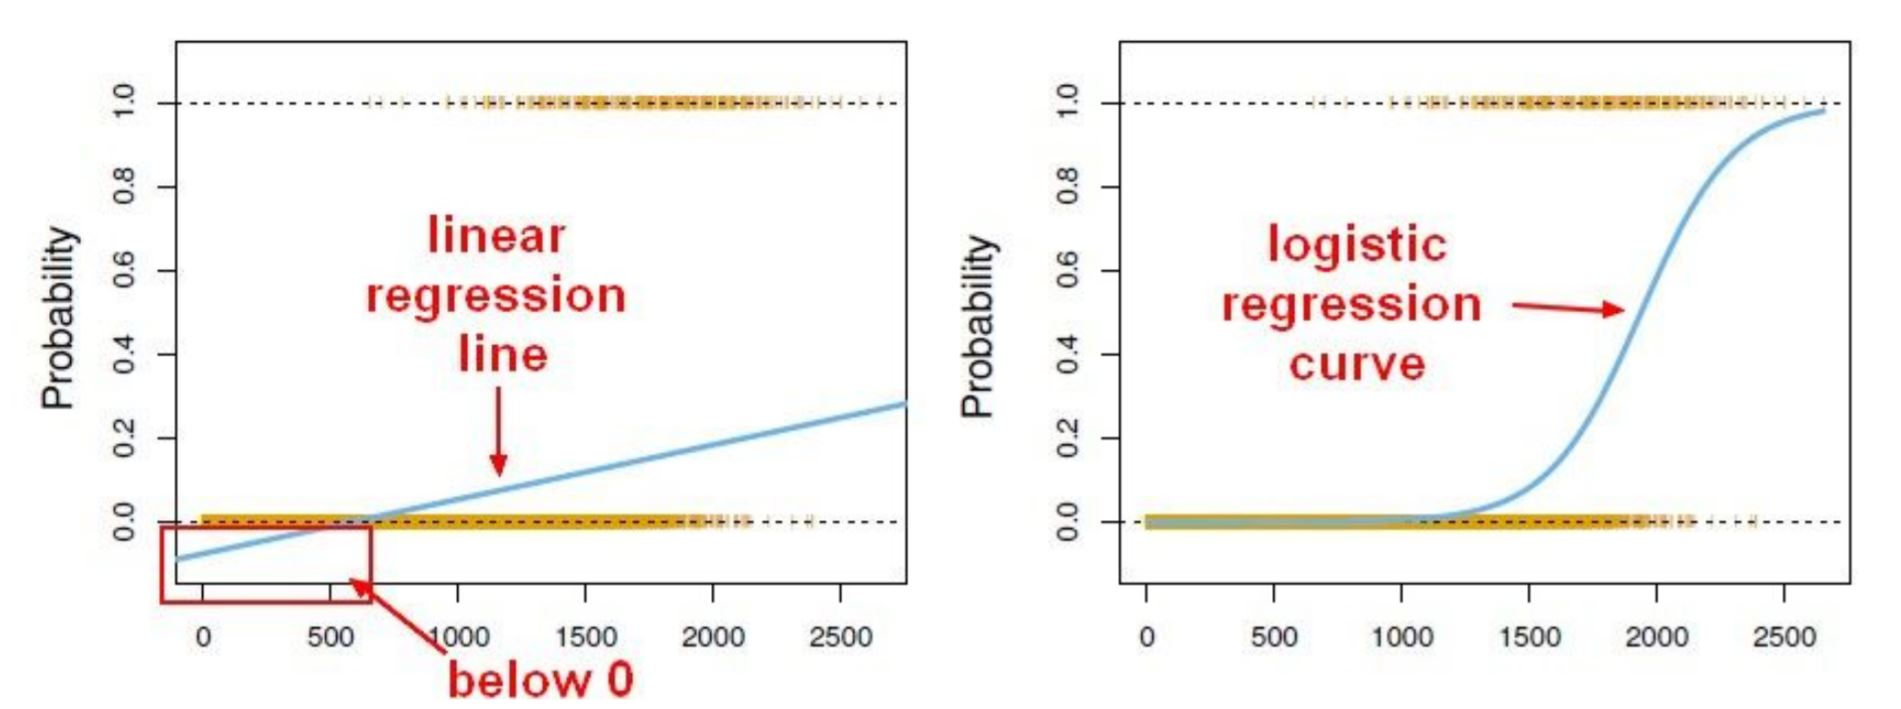
\includegraphics[width=0.9\textwidth]{pics/logistic_regression}
	\caption{Linear vs. Logistic regression} 
	\label{lin_log_regr}
\end{figure}
%         --------------------------------------

Sigmoid (aka Logistic) function takes in any value and outputs it between 0 and 1:
\[ \phi(z) = \frac{1}{1+e^{-z}}
\]
hence we can use Linear Regression solution $y=b_0+b_1 x$ and replace it into $z$: 
%          --------   FIGURE: sigmoid  -----------
\begin{figure}[htbp] 
	\centering
	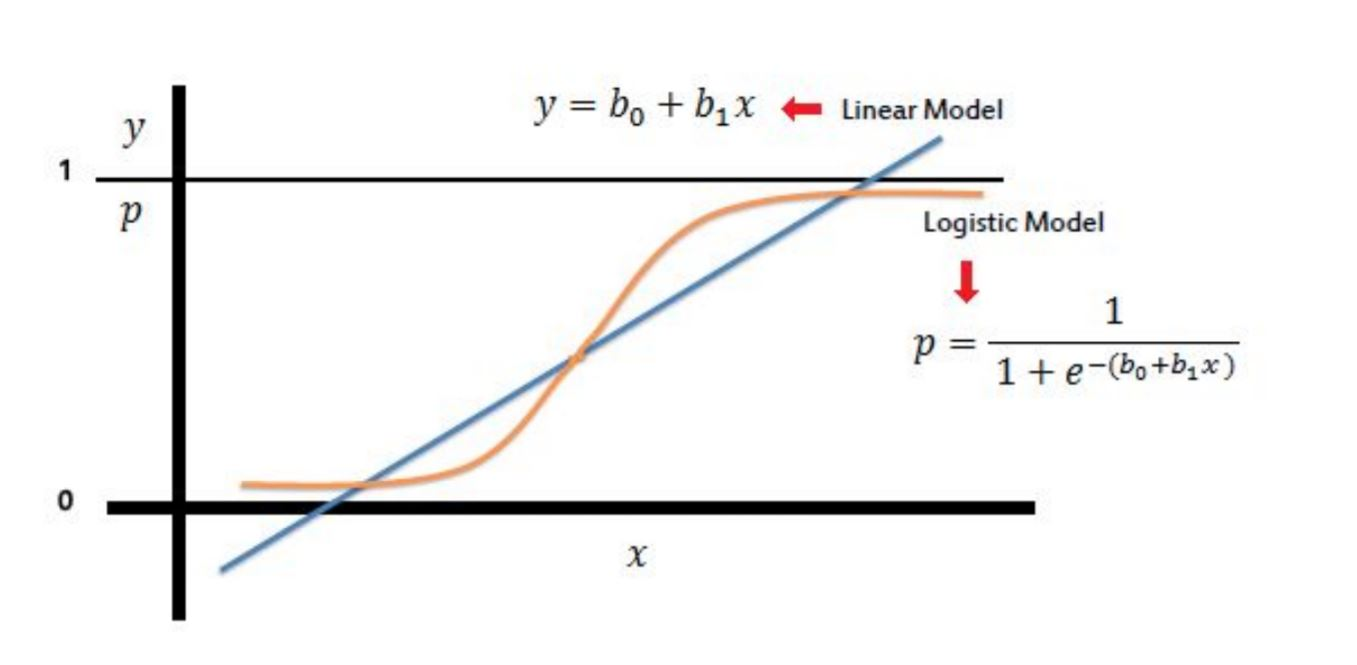
\includegraphics[width=0.7\textwidth]{pics/sigmoid}
	\caption{From linear to logistic}  
	\label{sigmoid}
\end{figure}
%         --------------------------------------

returning the \textbf{probability} (between 0 and 1) of belonging to a class: class 0 if prob below 0.5 and class 1 if above (see \ref{lin_log_regr}). 

Use \textbf{confusion matrix} to evaluate the model (e.g. disease vs. test) and true positive/true of the Logistic (or any classification model)
%          --------   FIGURE: confusion matrix  -----------
\begin{figure}[htbp] 
	\centering
	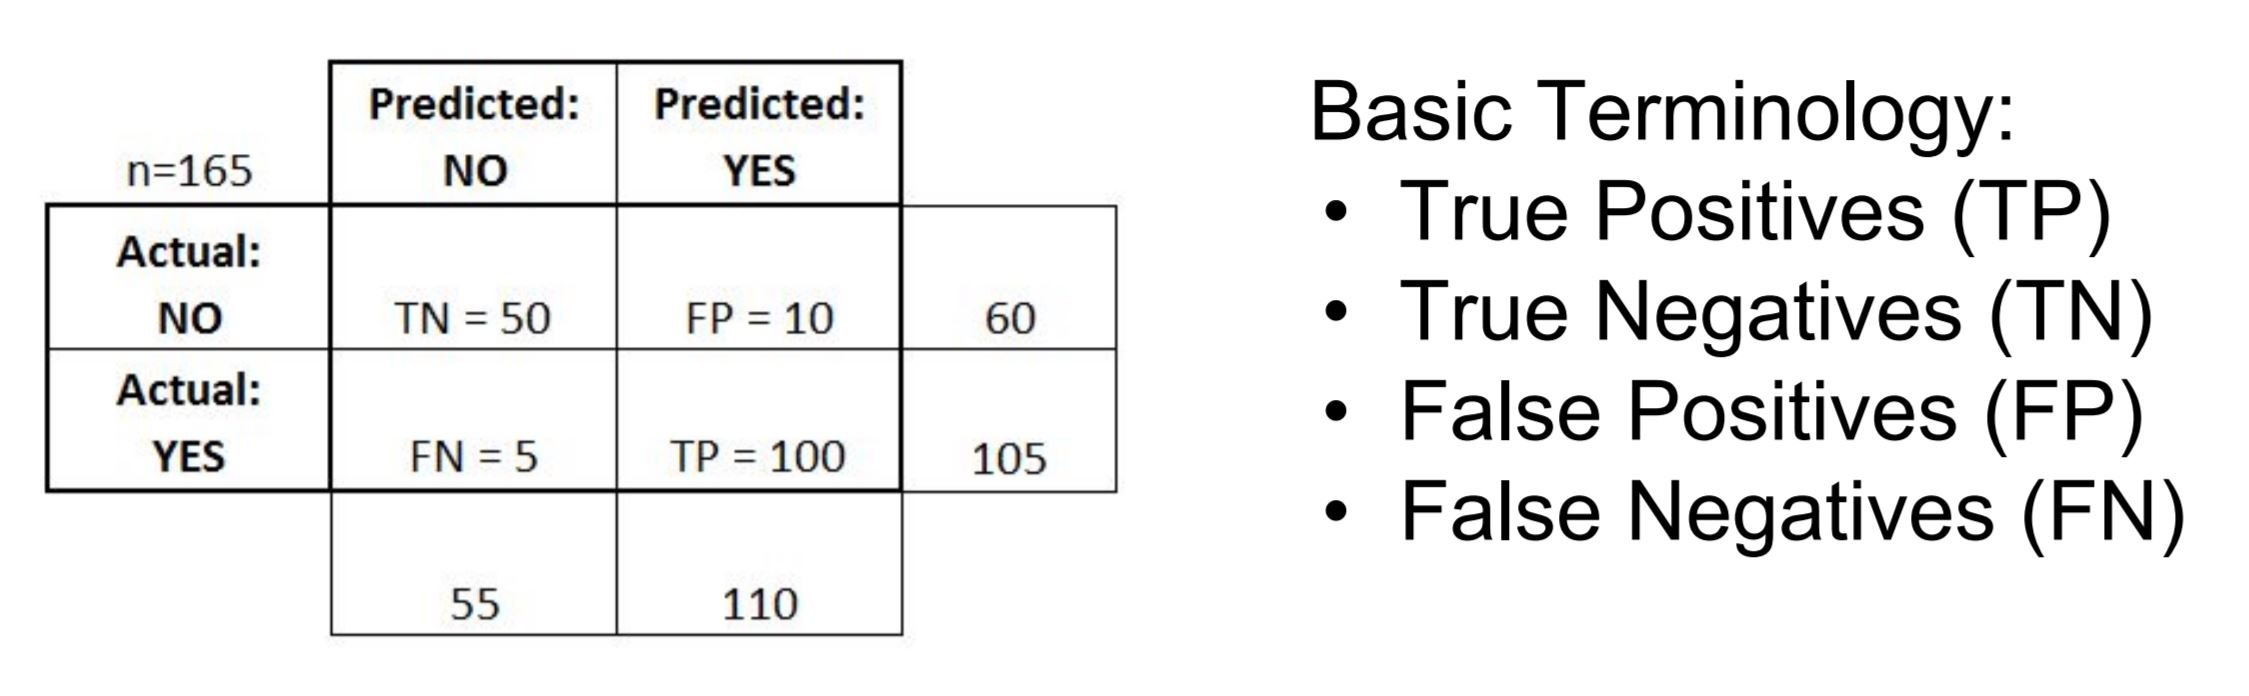
\includegraphics[width=0.7\textwidth]{pics/confusion_matrix}
	\caption{Confusion matrix}  
	%\label{XXXX}
\end{figure}
%         --------------------------------------

This is a \textit{short} list of rates that are often computed from a confusion matrix for a binary classifier:
\begin{itemize}
	\item \textbf{Accuracy}: (TP+TN)/tot = (100+50) / 165) = 0.91
	\item Error rate: (FP+FN)/tot = 1 - Accuracy
	\item \textbf{Recall} (or Sensitivity or True Positive Rate): TP/(\textit{actual} yes) = 100 / 105 = 0.95
	\item Specificity: TN/(actual no) = 50 / 60
	\item \textbf{Precision} TP/(\textit{predicted} yes) = 100 / 110 = 0.91
\end{itemize}
Use Precision and Recall rather than Accuracy rate (see 'accuracy paradox\footnote{For classification problems that are skewed in their classification distributions - e.g. if we had a 100 text messages and only 2 were spam and the rest 98 were not - accuracy by itself is not a very good metric. We could classify 90 messages as not spam (including the 2 that were actually spam, hence they would be false negatives) and 10 as spam (all 10 false positives) and still get a reasonably good accuracy score of 90\%. For such cases, precision and recall come in very handy. These two metrics can be combined to get the F1 score, which is weighted (harmonic) average of the precision and recall $F1\_score = 2 * \frac{prec * rec}{prec + rec}$} in wikipedia).

\begin{itemize}
	\item \textbf{Type I error} = False positive. \\ E.g. In a spam model, clearly worse to have a false positive (i.e. sending to the spam folder a non-spam email) than just the inconvenience of deleting a spam email that makes it to your inbox (false negative). Hence, we want to max \textbf{Precision} (up to 1. - how many spam emails correctely identified out of all predicted spam ones);
	\item \textbf{Type II error} = False negative \\ E.g. In a medical context, a false negative (sick people sent back home because diagnosed as healthy) is clearly worse than false positives (healthy individuals that have to do more tests). Hence we want to maximise \textbf{Recall} (how many diagnosed sick out of all sick people, e.g. precision 80\% but recall 95\%.).
\end{itemize}

Other \textit{evalutation metrics} are $F_{beta}$ (which is a generalisation of  $F1\_score$, see fig. \ref{F_beta_boundaries}) and Receiver Operating Characteristic ('ROC') curve (where the points are True Positive and True Negative Rate splitting, between (0, 0) and (1, 1))
%          --------   FIGURE: F_beta_boundaries  -----------
\begin{figure}[htbp] 
	\centering
	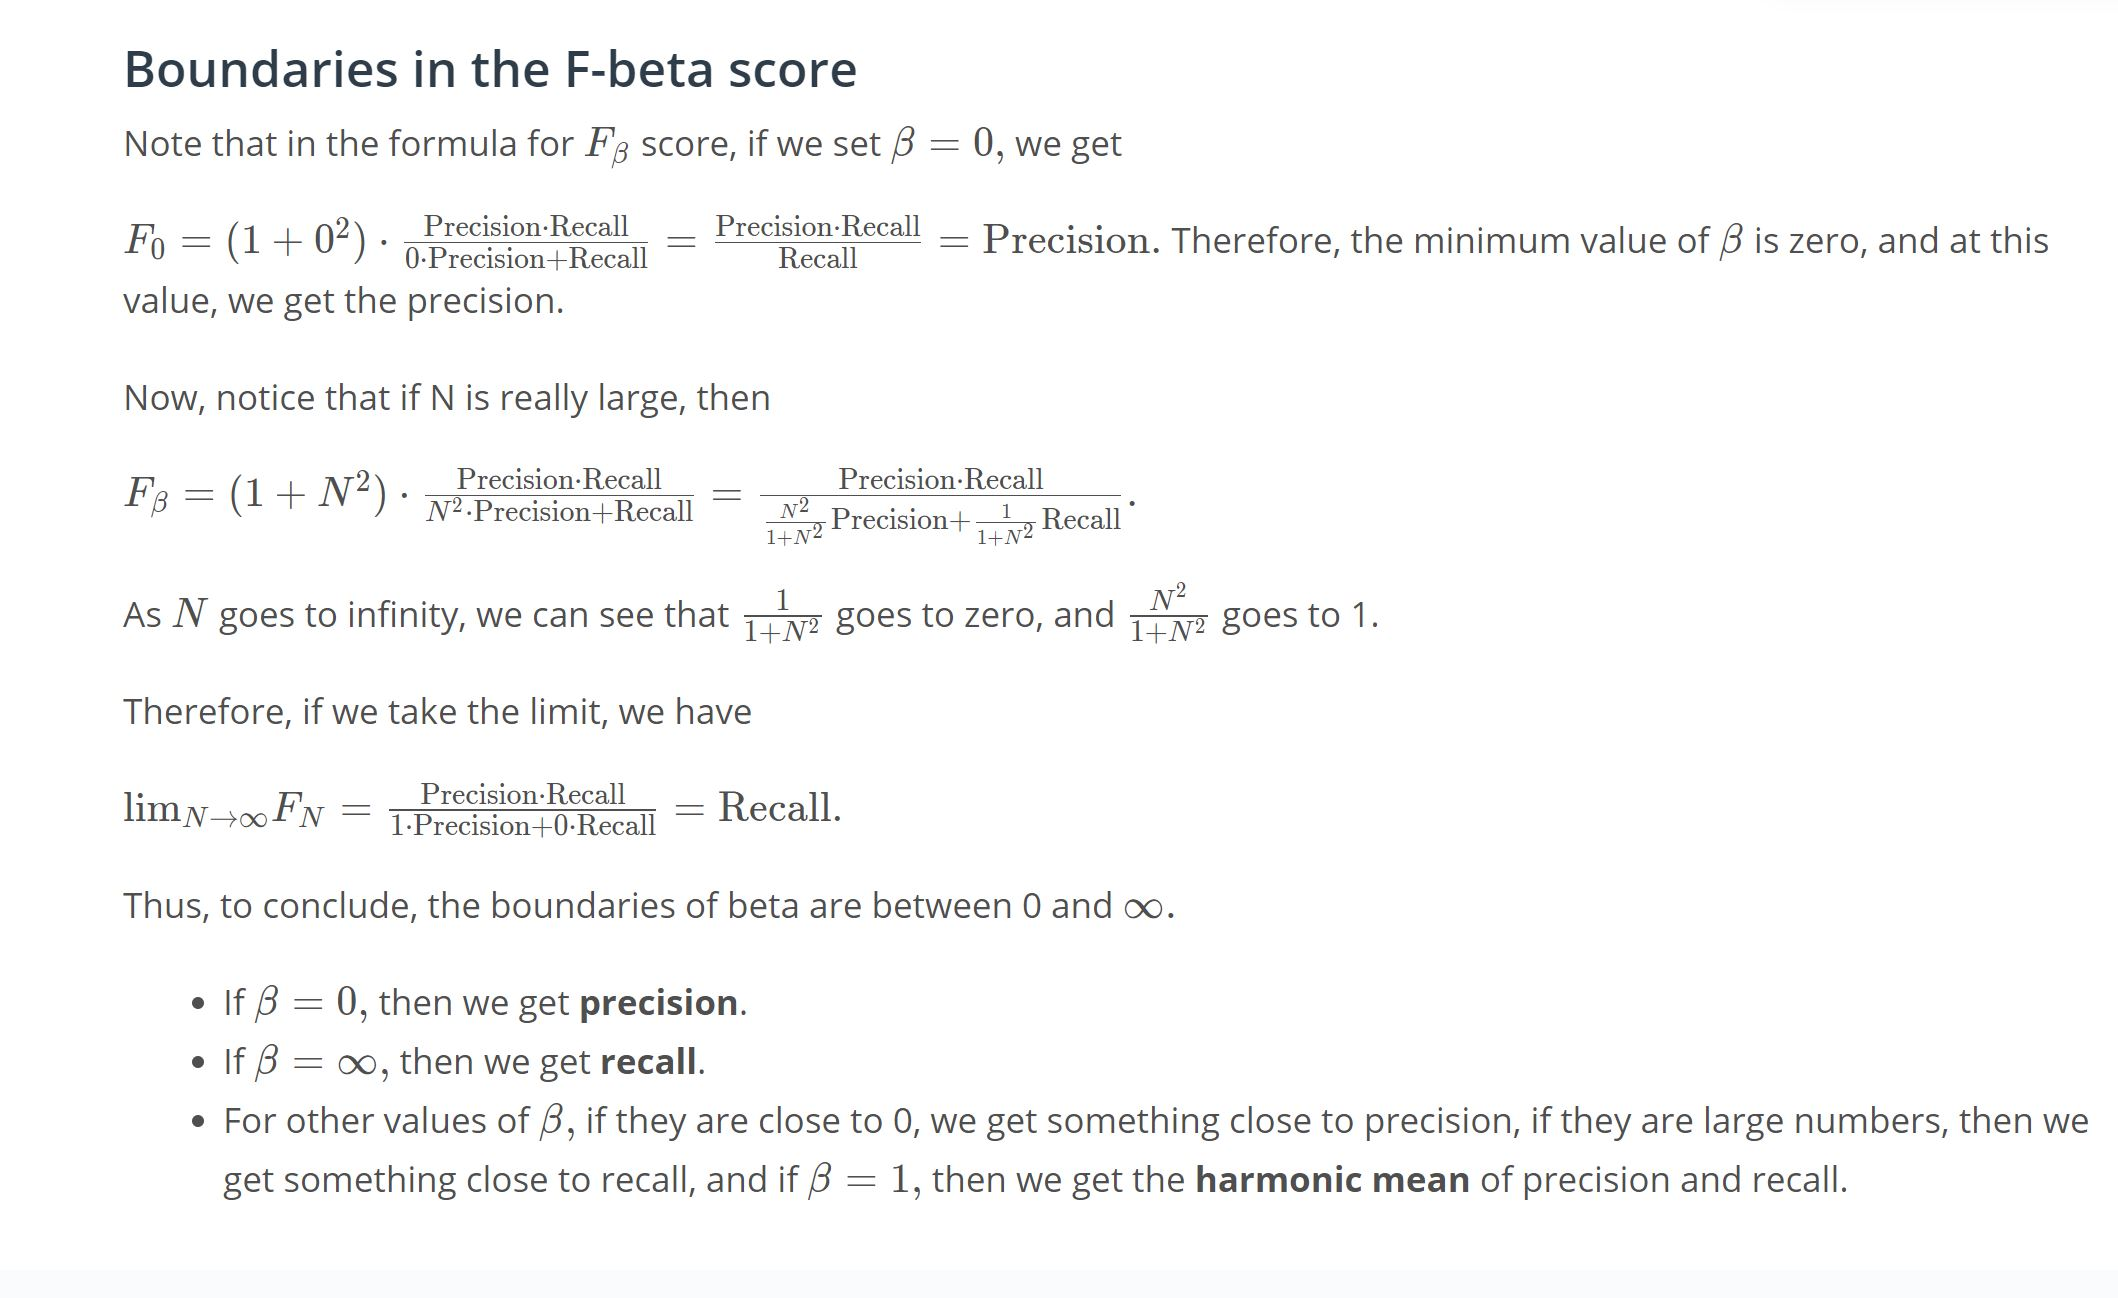
\includegraphics[width=0.85\textwidth]{pics/F_beta_boundaries}
	\caption{F beta}  
	\label{F_beta_boundaries}
\end{figure}
%         --------------------------------------

%          --------   FIGURE: ROC Curve -----------
\begin{figure}[htbp] 
	\centering
	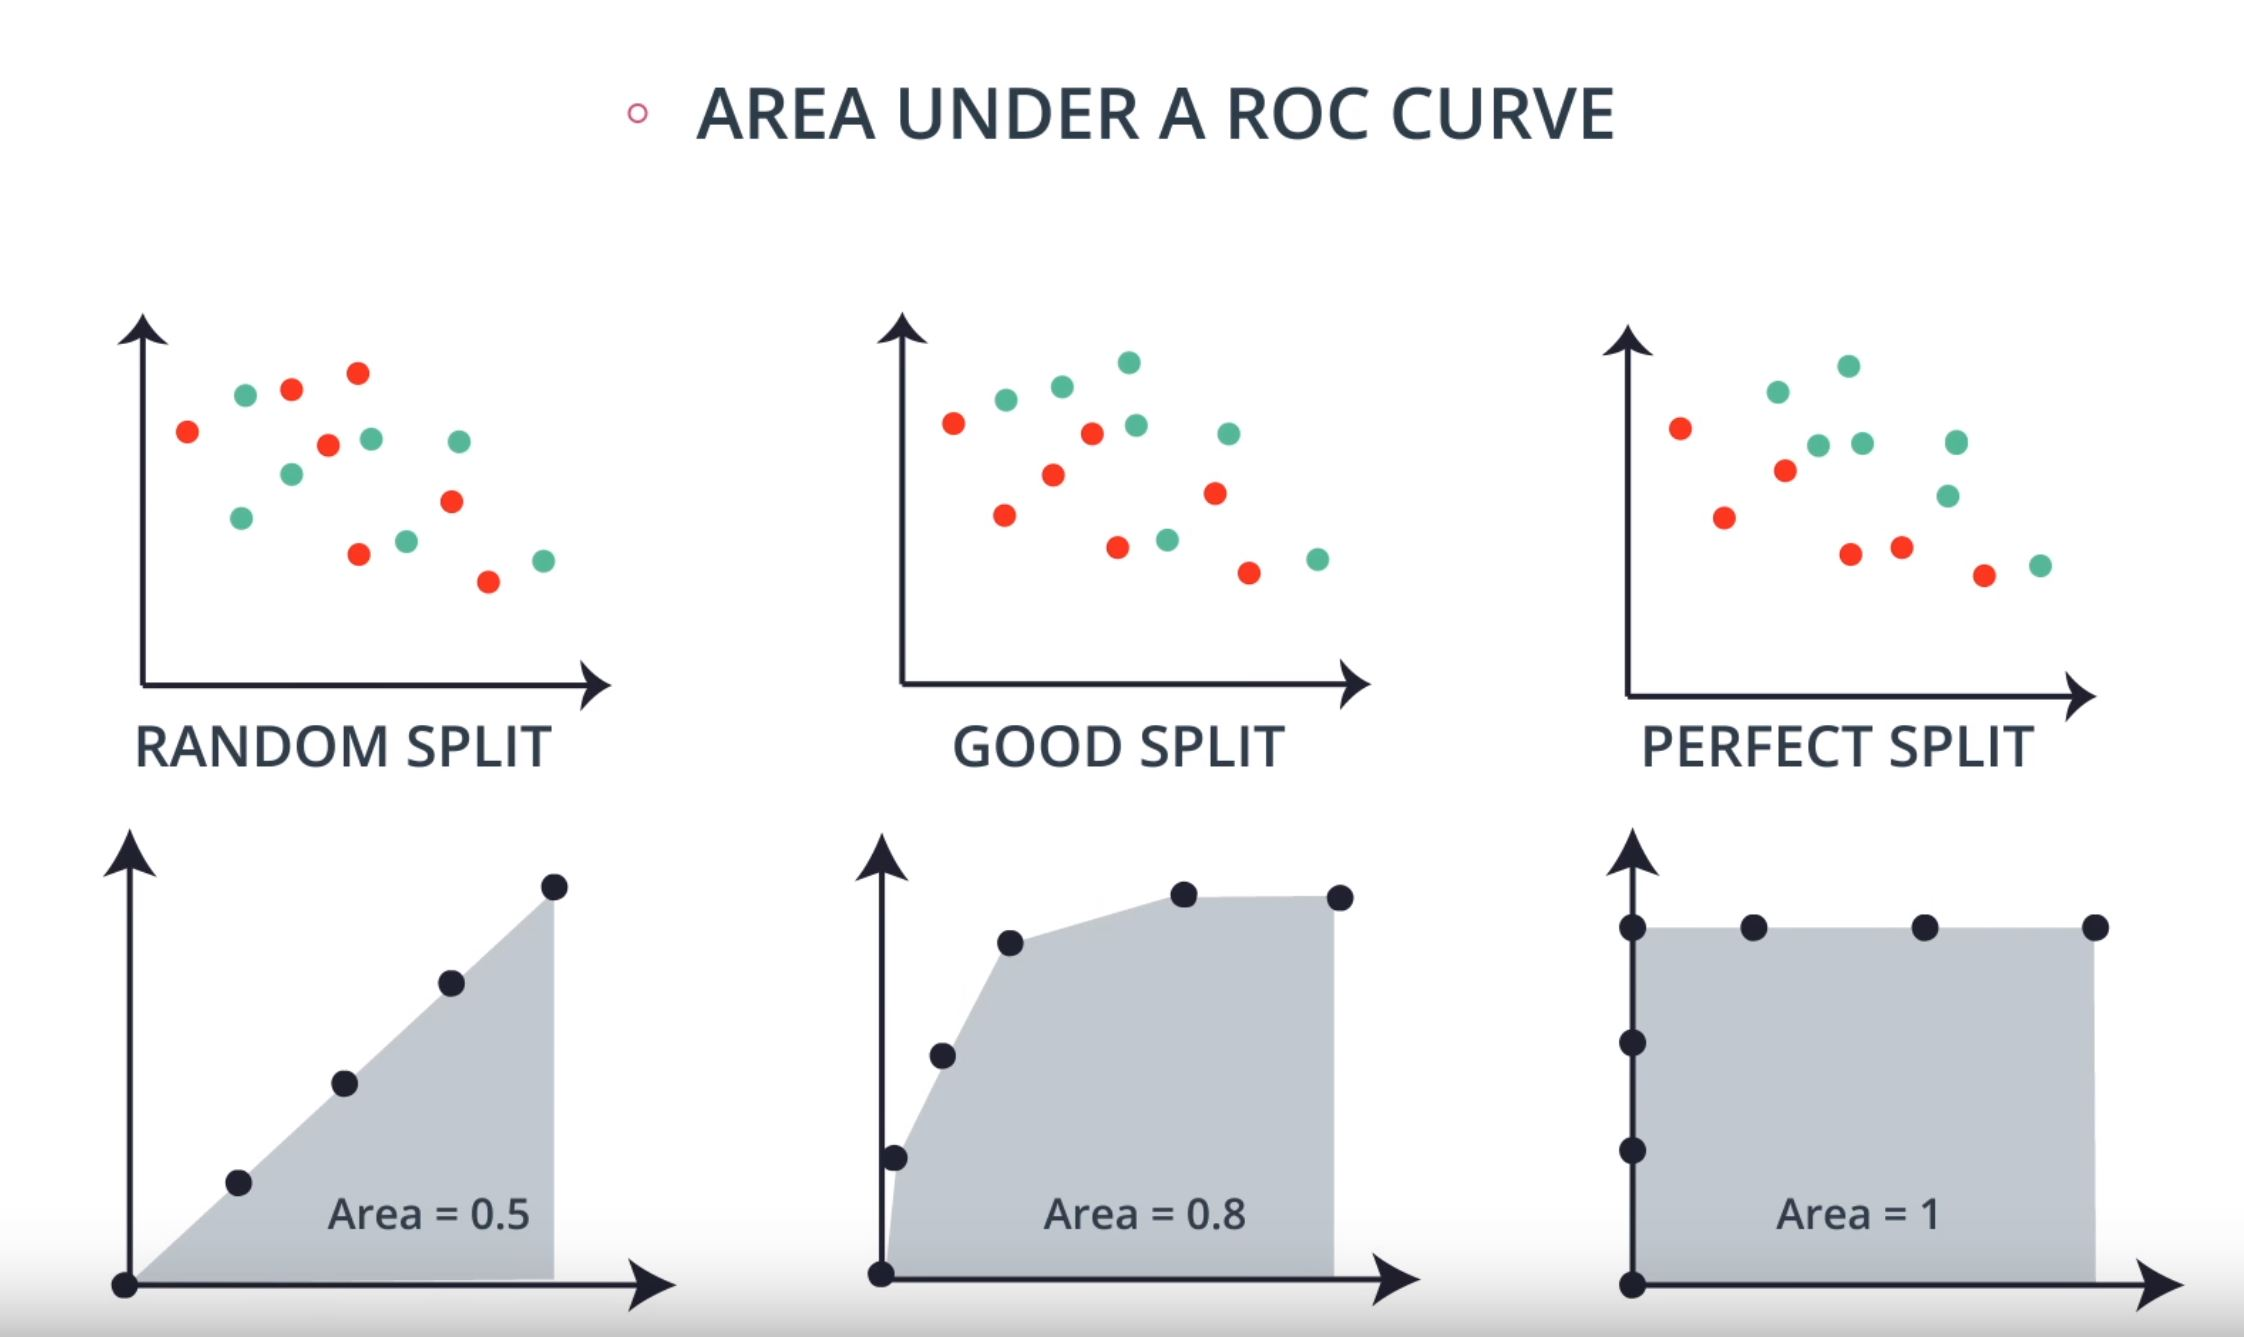
\includegraphics[width=0.7\textwidth]{pics/ROC_curve}
	\caption{ROC curve}  
	\label{ROC_curve}
\end{figure}
%         --------------------------------------

Learning curves plots the prediction accuracy/error vs. the training set size (ie: how better does the model get at predicting the target as you the increase number of instances used to train it)

And now the code:
\begin{lstlisting}
train = pd.read_csv('titanic_train.csv')  # load data

# heatmap to visualise missing data
sns.heatmap(train.isnull(),yticklabels=False,cbar=False,cmap='viridis')

# 1. visualise data
sns.set_style('whitegrid')
sns.countplot(x='Survived',hue='Sex',data=train,palette='RdBu_r')
sns.countplot(x='Survived',hue='Pclass',data=train,palette='rainbow')
sns.distplot(train['Age'].dropna(),kde=False,bins=30) # or
train['Age'].hist(bins=30)  # NB: no .dropna() needed

# 2. clean data (wealthier passengers -> older)
plt.figure(figsize=(12, 7))
sns.boxplot(x='Pclass',y='Age',data=train,palette='winter')

def impute_age(cols):
	Age = cols[0]
	Pclass = cols[1]
	if pd.isnull(Age):  # data missing
		if Pclass == 1:
			return 37
		elif Pclass == 2:
			return 29
		else:
			return 24
	else:
		return Age

 # apply fnct - NB: axis=1
train['Age'] = train[['Age','Pclass']].apply(impute_age,axis=1)

 # drop a useless col and na rows
train.drop('Cabin',axis=1,inplace=True)
train.dropna(inplace=True)

# 3. convert categorical vars into dummy variables 
# dummies for a series, then concat axis=1
sex = pd.get_dummies(train['Sex'],drop_first=True)
# or, alternatively, train['Sex'] = train.Sex.map({male:1, female:0})
embark = pd.get_dummies(train['Embarked'],drop_first=True)
 # remove unnecessary cols
train.drop(['Sex','Embarked','Name','Ticket'],axis=1,inplace=True)
 # get new cols in (NB: axis=1)
train = pd.concat([train,sex,embark],axis=1)

# alternative: apply dummies to the col & rtrn all
final_data = pd.get_dummies(df_loans,columns=["colum_name"],drop_first=True)

# 4. build model
 # train
X_train, X_test, y_train, y_test = 
	 train_test_split(train.drop('Survived',axis=1), 
		train['Survived'], test_size=0.30, random_state=101)
 # build 		
from sklearn.linear_model import LogisticRegression
logmodel = LogisticRegression()
logmodel.fit(X_train,y_train)

predictions = logmodel.predict(X_test)

 # evaluate
from sklearn.metrics import classification_report
print(classification_report(y_test,predictions))
\end{lstlisting}

%%%%%%%%
To recap, the \textbf{evaluation metrics} are:
\begin{itemize}
	\item \underline{regression}: mean absolute error (but not differentiable), mean square error, R2.
	\item \underline{classification}: accuracy (but note for skew distributions), precision and recall, $F1\_score$ and its generalisation, ROC.
\end{itemize}

%%%%%%%%%%%%%%%%%%%%%%%%%%%%%%%%%%%%%%%%%%%%%%%%%%%%%%
\subsection{Bayes Learning} \label{Bayes} 

\subsubsection{Naive Bayes}
The probabilistic model of naive Bayes classifiers is based on Bayes' theorem, and the adjective \textit{naive} comes from the fact that the algorithm considers the features (or attributes) that it is using to make the predictions to be mutually \textit{independent}, which may not always be the case (e.g. a naive Bayes spam filter considers the frequency, but not the order of the words). In practice, the independence assumption is often violated, but naive Bayes classifiers still tend to perform very well under this unrealistic assumption - especially for small sample sizes.

One of the major advantages that Naive Bayes has over other classification algorithms is its ability to handle an extremely large number of features. For example, in a spam detector algorithm each word is treated as a feature and there are thousands of different words. Also, it performs well even with the presence of irrelevant features and is relatively unaffected by them. The other major advantage it has is its relative simplicity. Naive Bayes' works well right out of the box and tuning it's parameters is rarely ever necessary, except usually in cases where the distribution of the data is known. It rarely ever overfits the data. Another important advantage is that its model training and prediction times are very fast for the amount of data it can handle. 

Example, if $h = Cancer$ and $D (data) = \text{positive test}$:
\[ \underbrace{P(Cancer|Pos)}_{\text{a posteriori}} = \frac{ P(Pos|Cancer) \; \overbrace{P(Cancer)}^{\text{a priori}} }{P(Pos)} 
\]
%          --------   Bayes:   -----------
\begin{figure}[htbp] 
	\centering
	\includegraphics[width=0.9\textwidth]{pics/bayesian_learning}
	\caption{Bayes learning} 
	\label{bayesian_learning}
\end{figure}
%         --------------------------------------


\begin{lstlisting}
from sklearn.naive_bayes import MultinomialNB, GaussianNB
naive_bayes = MultinomialNB()  # GaussianNB
naive_bayes.fit(training_data, y_train)
predictions = naive_bayes.predict(testing_data)
\end{lstlisting}


Note that the final expression is the OLS in fig. \ref{bayesian_learning2} or perceptron: if Hp is linear and errors are i.i.d and Gaussians, we recover regression (e.g. $x_i$ are heights and $d_i$ the weights of people)

%          --------   Bayesain Learning 2  -----------
\begin{figure}[htbp] 
	\centering
	\includegraphics[width=0.9\textwidth]{pics/bayesian_learning_2}
	\caption{Bayes learning 2} 
	\label{bayesian_learning2}
\end{figure}
%         --------------------------------------

Note that $lg$ in fig. \ref{bayesian_learning3} is the $log$ in base $2$ (number of bits). This is showing the link to entropy (error/wrong labels and size of hp): you want to find the simplest hypothesis that minimise the errors (usually the two terms are a trade-off: complicated hypothesis tend to reduce errros and vice-versa). This is called the "minimum description lenght". This justifies, somehow, the Occam's razor.
%          --------   Bayesain Learning 3  -----------
\begin{figure}[htbp] 
	\centering
	\includegraphics[width=0.9\textwidth]{pics/bayesian_learning_3}
	\caption{Minimum description lenght} 
	\label{bayesian_learning3}
\end{figure}
%         --------------------------------------

Once we find $P(h|D)$ we really need to get a classification: see formula in fig \ref{bayesian_learning4} 
%          --------   Bayesain Learning 4  -----------
\begin{figure}[htbp] 
	\centering
	\includegraphics[width=0.9\textwidth]{pics/bayesian_learning_4}
	\caption{Bayes classification} 
	\label{bayesian_learning4}
\end{figure}
%         --------------------------------------

\subsubsection{Belief Networks}
Belief Networks (also called Bayes Nets or Bayesian Networks or Graphical Models) represent - graphically (via nodes and branches) - conditionally probabilities on events - and any joint probability comes from multiplying such conditional ones. If not independent, then it grows exponentially since you get more branches going into same event/node. Dependence does not mean causality (obviously). \textit{Topological} order (for sampling the joint distribution): it must be acyclic (you need to go from parent(s) to children).

%          --------   Bayesain Learning 4  -----------
\begin{figure}[htbp] 
	\centering
	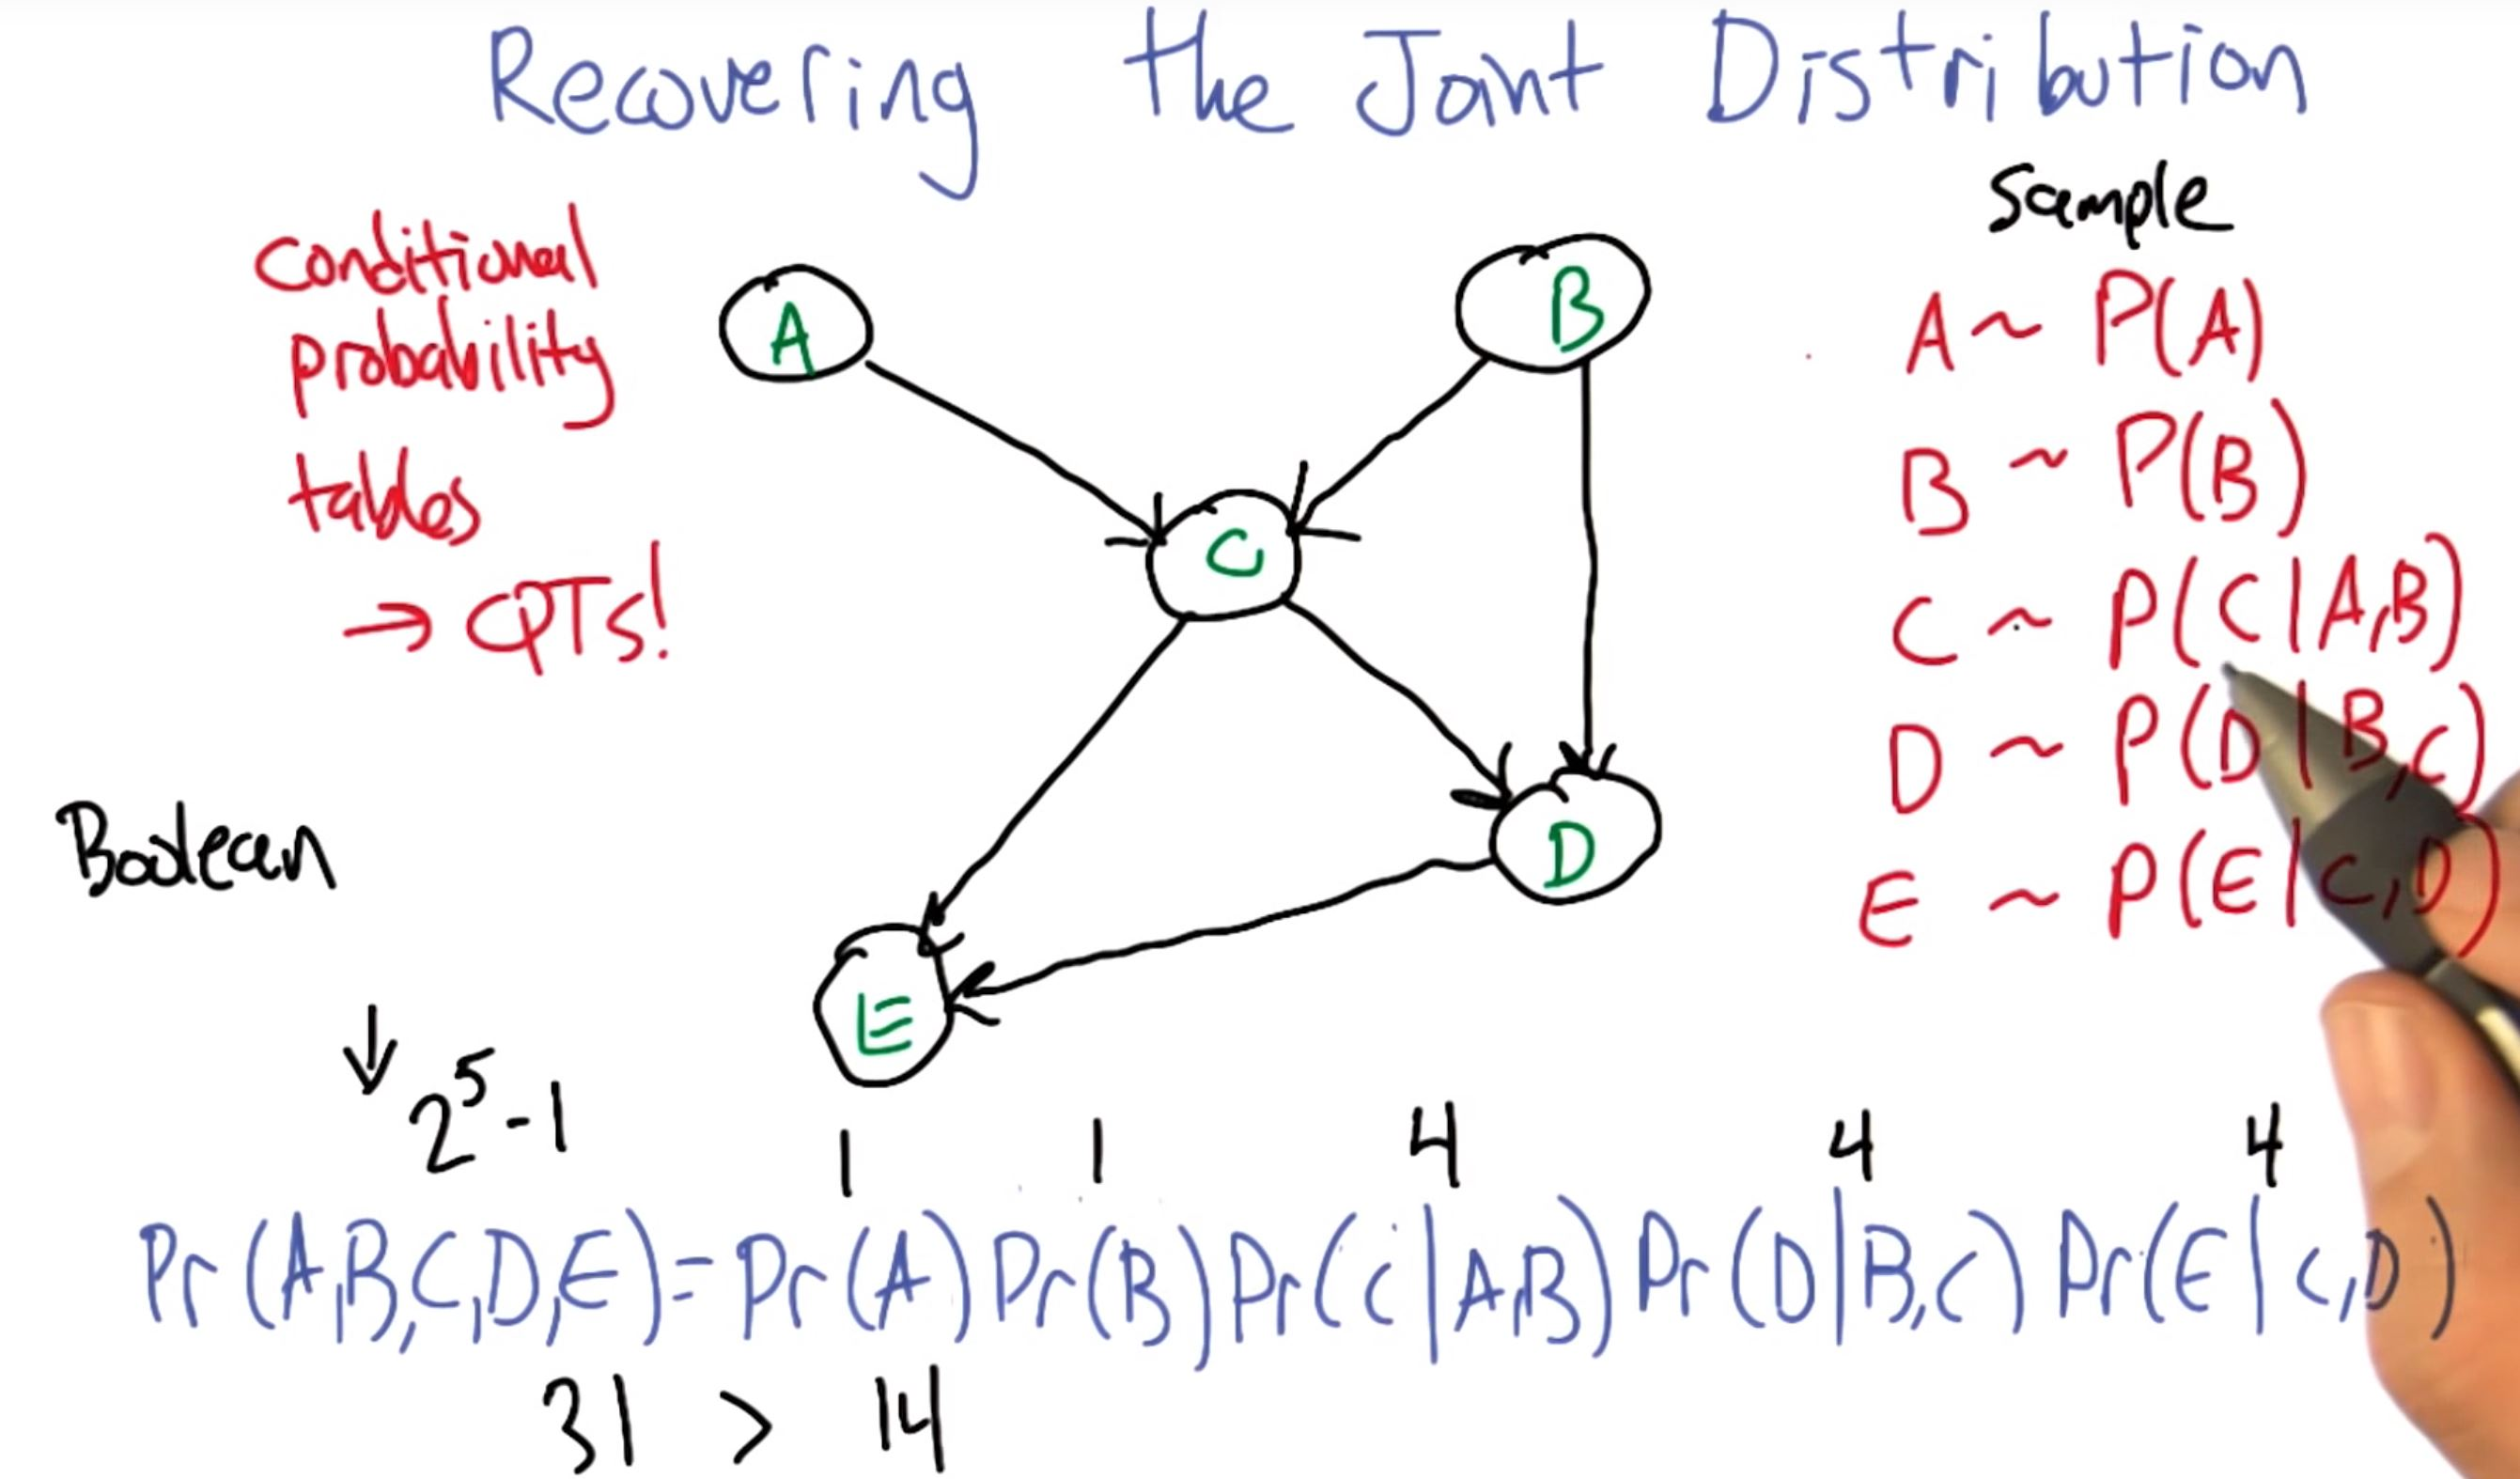
\includegraphics[width=0.9\textwidth]{pics/belief_network1}
	\caption{Sampling} 
	\label{belief_network1}
\end{figure}
%         --------------------------------------
Belief networks can be useful for approximate inference (simulate/generate some samples to infer 'reverse' conditional probability - easier to solve and faster), visualitation (get a fee), simulation of complex process. 

%          --------   Bayesain Learning 5  -----------
\begin{figure}[htbp] 
	\centering
	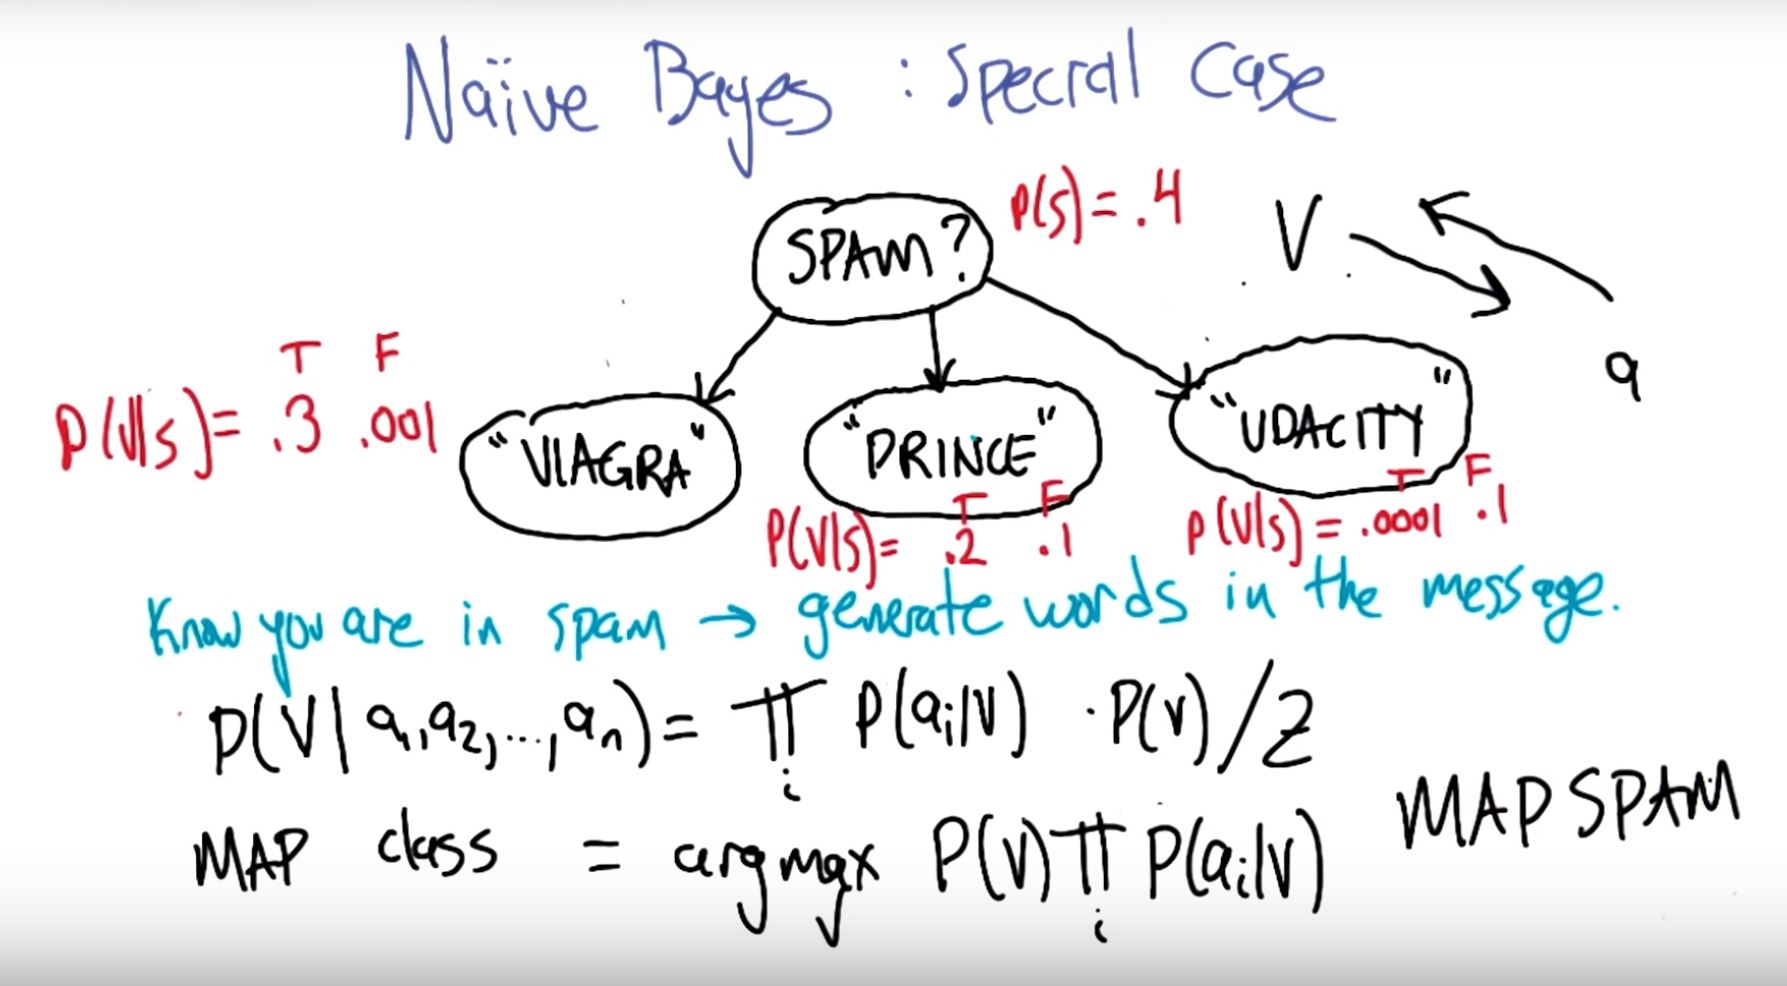
\includegraphics[width=0.9\textwidth]{pics/Bayesian_special_case}
	\caption{Bayes SPAM (Bayes link to classification)} 
	\label{Bayesian_special_case}
\end{figure}
%         --------------------------------------

Why Naive Bayes is cool:
\begin{itemize}
	\item inference (in any direction) is cheap - linear rather than exponential (just using Bayes formula);
	\item few parameters;
	\item estimate parameters with labelled data: $Pr(attr_i | Class) = \frac{\# \, attr_{i,C}}{\# \, C}$ (one unseen attribute may spoil the whole classificztion, hence 'smooth' applied or the inductive bias);
	\item connect inference and classification;
	\item empirically succesful. Even if the model does not model interrelationships beetween atributes, it is still able to preserve the order (which in classification is what we care about).	 
\end{itemize}

\subsubsection{Bag of Words}
 Bag of Words(BoW) is a concept used to specify the problems that have a collection of text data that needs to be worked with. The basic idea of BoW is to take a piece of text and count the frequency of the words in that text. It is important to note that the BoW concept treats each word individually and the order in which the words occur does not matter (it is a 'naive' Bayes, indeed).

From scratch:
\begin{lstlisting}
from import CountVectorize
# TO BE COMPLETED
\end{lstlisting}

From scratch:
\begin{lstlisting}
#
#	INSERT 
#
\end{lstlisting}

%%%%%%%%%%%%%%%%%%%%%%%%%%%%%%%%%%%%%%%%%%%%%%%%%%%%%%
\subsection{K Nearest Neighbours} \label{K_Nearest_Neighbours} 
KNN is a (non parametric) classification (or regression, see below) algorithm based on a simple principle, first one stores all the data (training) and then follows the steps below for the prediction:
\begin{itemize}
	\item calculate distance from $q$ to all points $x_i$ in your data,
	\item sort the data by increasing distance from $q$ (or some other similarity: our domain knowledge),
	\item predict $q$ using majority label of the 'K' closest pointss.
\end{itemize}
Example: think about cost label of a house (e.g. expensive, medium, cheap) vs. some nearby houses we know the price/labels of - how many houses ('K') are to be considered in a neighbourhood? say e.g. 5, calculate the distances, rank and get closest 5 houses, predict our unknown-label house using the majority label of such 5 closest houses.  

The choice of K will clearly affect what class new point is assigned to (k=1 is very noisy, ...) as it does the choice of distance (e.g. Euclidean vs. L1-norm / Manhattan). Simple, but not good for large data sets and for categorical features.

Preference bias of KNN (our belief of what makes a good Hp):
\begin{itemize}
	\item locality (near points are \underline{similar}: \textbf{distance}, e.g. Euclidean vs. L1),
	\item smoothness (\textbf{averaging}),
	\item all features matter \underline{equally} (think of using KNN regression on a function that was actually $y=x_1^2 + x_2$, clearly $x_1$ more important and KNN will not be that good).
\end{itemize}

Why standardise the variables: the KNN classifier predicts the class of a given test observation by identifying the observations that are nearest to it, therefore the scale of the variables matters (large scale variables will have a much larger effect on the distance and hence on the KNN classifier).
\begin{lstlisting}
# 1. read data
df = pd.read_csv("Classified Data",index_col=0)

# 2. standardise variables (import, fit and transform)
from sklearn.preprocessing import StandardScaler
scaler = StandardScaler() # initialise
scaler.fit(df.drop('TARGET CLASS',axis=1)) # targ class = 0 or 1
scaled_features = scaler.transform(df.drop('TARGET CLASS',axis=1))
# scaled_feature is an array now, so we re-create df
# note: scaled_fatures will also work in train or KNN algo
df_feat = pd.DataFrame(scaled_features,columns=df.columns[:-1])

# 3. build model
  # train test split
from sklearn.model_selection import train_test_split
X_train, X_test, y_train, y_test = 
	train_test_split(scaled_features,df['TARGET CLASS'],
		test_size=0.30)

 # using KNN (starting with K =1)
from sklearn.neighbors import KNeighborsClassifier
knn = KNeighborsClassifier(n_neighbors=1)  # K = 1
knn.fit(X_train,y_train)
pred = knn.predict(X_test)
 
 # evaluate
from sklearn.metrics import classification_report,confusion_matrix
print(confusion_matrix(y_test,pred))
print(classification_report(y_test,pred))
# from sklearn.metrics import accuracy_score, precision_score, recall_score, f1_score
# print(accuracy_score(y_test, pred))

 # choose right K value
error_rate = []
for i in range(1,40):  # will take some time
	knn = KNeighborsClassifier(n_neighbors=i)
	knn.fit(X_train,y_train)
	pred_ = knn.predict(X_test)
	error_rate.append(np.mean(pred_ != y_test))

plt.figure(figsize=(10,6))
plt.plot(range(1,40),error_rate,color='blue', ls='dashed', 
  marker='o', markerfacecolor='red', markersize=10)
plt.title('Error Rate vs. K Value')
plt.xlabel('K')
plt.ylabel('Error Rate')
\end{lstlisting}
You see that after, say, K$>$20 the error rate just tends to hover around, say, 0.06-0.05. Get confusion matrix and classification report with say K=20 and compare vs. those of K=1.

Instance-based learning in general
Advantage: (i) it does not forget data (e.g. in regression, we fit the model to the training data but we don't use it anymore), (ii) fast and (iii) simple. But: (i) no generalisation and (ii) overfit.

\textit{Curse of dimensionality}: as the number of features or dimensions grows, the amount of data we need to generalise accurately grows \underline{exponentially}. E.g. 10 points in 1 dim, become 100 in 2-dim and 1000 in 3-dim... This is an issue for KNN only.

%%%%%%%%%%%%%%%%%%%%%%%%%%%%%%%%%%%%%%%%%%%%%%%%%%%%%%
\subsubsection{KNN regression}
Above we saw the KNN classifier, here we look at the KNN regression (i.e. y's are numbers rather than labels) - this is a non-parametric regression, we predict y as the \textit{mean} of y's rather the more frequent label (i.e. regression: mean of $y_i$ in NN vs. classification: vote/plurality/majority of the $y_i$).

LOOK AT MY NOTES

\subsubsection{Kernel regression}
Difference: here we weight the contribution of each $x_i$ we have based on how far away from $x$ at hand, whilst in KNN regression every $x$ is essentially equally-weighted. For example, we can replace the average with locally-weighted regression or even Neural Networks or other algorithms.

%%%%%%%%
To recap:
\begin{itemize}
	\item parametric: if problem is biased, meaning that you have an idea of the relationship in terms of functional form, then use a parametric model/approach (e.g. how far a cannon is going to shoot, given the angle);
	\item non-parametric: for un-biased problems, when you have no idea of the functional forms, then best to use a non-parametric approach (e.g. bees population as function of the food richness). More data-intensive since you have to store all data, but no need to guess the form of the solution.
\end{itemize}


In \textbf{eager} learners, e.g. Naive Bayes or regression, the computationally most expensive step is the model building (learning the model from a training dataset) whereas the classification of new instances is relatively fast (once model is learned).

\textbf{Lazy} learners, like KNN, instead memorise and re-evaluate the training dataset for predicting the class label of new instances. Here is the model building step that is relatively fast, whilst the actual prediction is typically slower due to the re-evaluation of the training data. Another disadvantage of lazy learners is that the training data has to be retained, which can also be expensive in terms of storage space.

Note that - assuming sorted data points - (i) in linear regression the learning runnig time is $n$ (filling matrix and inverting), whilst querying is constant (fast), (ii) instead for KNN is almost the reverse: learning speed is constant but query is $ln(n)$. 

Every time a new instance is encountered, KNN would evaluate the k-nearest neighbours in order to decide upon a class label for the new instance, e.g., via the majority rule (i.e., the assignment of the class label that occurs most frequently amongst the k-nearest neighbors).

%%%%%%%%%%%%%%%%%%%%%%%%%%%%%%%%%%%%%%%%%%%%%%%%%%%%%%
\subsection{Decision Trees and Random Forests}
E.g. shall I enter this restaurant or not? possible instances/features: type of cuisine (Italian, French, ...), atmosphere (fancy, casual, ...), occupied, costs (discrete or number), hungry?, raining (would like to stop now), ... 

Representation: what is a decision tree vs. algorithm (latter is how you implement such representation).

Representation: a tree is made-up of
\begin{itemize}
	\item Nodes: defined by the value of a certain \textit{attribute}, using questions for further splits or arrival point; 
	\item Edges or branches: outcome of a split to the next node (represent \textit{values}, i.e. answers to the question in preceding node)
\end{itemize}
also nodes are of two kinds:
\begin{itemize}
	\item Decision nodes (that topmost called root node): node that performs splits (usually drawn as a circle, it has two or more branches);
	\item Leaf notes: \textit{terminal} nodes that represent the outcome(s) (usually drawn as a boxe or just the end-result), they've got just one branch to a decision node or no branches (for the final ones).
\end{itemize}

The goal is to narrowing possibilities in getting the right class. Algorithm: pick best attributes and ask questions (e.g. best: halving possibilities), follow answer path and repeat (questions get more and more specific) until got an answer. 

\textbf{Entropy} (that measures the homogeneity of a data set, from zero to the $log_2$ of different classes\footnote{E.g. for two classes: if all samples belong to one class then entropy is zero (no uncertainty), if data equally split between the two classes ($p_1 = p_2 = 0.5$) then entropy is 1 (the max for two classes). You can think of it as a parable with max of 1 at p=0.5 and minima of zero when p is either 0 or 1,}) and Information Gain (how well an attribute splits the data into groups based on classification: it measures the reduction in entropy that results from partitioning the data on an attribute) are the Mathematical Methods of choosing the best split (ref Ch 8 of Gareth et al):
\[ Gain(S, A) = Entropy(S) - \sum_v \frac{|S_v|}{|S|} Entropy(S_v)
\]
where $S$ is the collection of training examples, $A$ is the attribute, $v$ is a particular class. And, finally, Entropy is $-\sum_v p(v) \,log_2[p(v)]$ (a measure of randomness or information). Recall that p(v) is the fraction of examples in class v. 

In short, constructing a decision tree is all about finding attribute that returns the highest Information Gain (i.e., the most homogeneous branches). Note that in sklearn DecisionTreeClassifier the default criterion is the Gini index ('gini'), rather than the information gain ('entropy').  

\textit{Expressiveness} (i.e. space of our hypothesis): n-or linear tree vs. n-xor\footnote{Difference: 'xor' is only true when either $x or $y is true, but not both (as instead for 'or'), i.e. is exclusive vs. inclusive.} (e.g. odd parity: true if odd no. of T) tree nodes are $o(2^n)$, very hard (being exponential fnct). 
Suppose we have $n$ boolean attributes and output is boolean, how many trees (or rows in a truth table) are needed? rows are $2^n$ and trees are even more: $2^{2^n}$ (which is not $4^n$ and after just n=6 already explodes). 

Example of algorithm (implementation): ID3 - a top-down, greedy search through the space of possible branches with no backtracking. ID3 uses Entropy and Information Gain to construct a decision tree:
\begin{itemize}
	\item Calculate entropy of the target.
	\item The dataset is then split on the different attributes. The entropy for each branch is calculated. Then it is added proportionally, to get total entropy for the split. The resulting entropy is subtracted from the entropy before the split, the result is the Information Gain or decrease in entropy. 
	\item choose the attribute with the largest information gain as decision node; repeat for each new branch (if the entropy of the branch is zero 0 all yes or all no -  is a leaf node, continuous untill all leaf nodes, i.e. all classified.)
\end{itemize}


ID3 biases. Restriction bias (hypothesis: considering only decision trees, not an infinite number but a well defined set) and preference bias (what we prefer from the hypothesis set vs. another). Inductive bias -> algo preferences: good splits at top, correct over incorret, shorter tres.

Other considerations for decision trees.
\begin{itemize}
	\item continuous attributes? what about for example 'age', we can use a range (e.g. a node with $20 \le age<30$ and since it is a continuous attribute we may ask again another question on it e.g. $age<20$).
	\item when do we stop? when everything correctly classified, no more (discrete) attributes, no overfitting (noise always inside data: use cross-validation or expand the tree until error does not drop much or 'pruning', which is collapsing the leaves if error small enough).
	\item regression: how to adapt a tree to continuous outputs. You need a different splitting criterion than information gain, e.g. variance, average of linear output.
\end{itemize}


A tree separates the space (decision boundaries), see \ref{tree_linear_separator}: two questions separates the space with two lines.
%          --------   FIGURE: tree_linear_separator  -----------
\begin{figure}[htbp] 
	\centering
	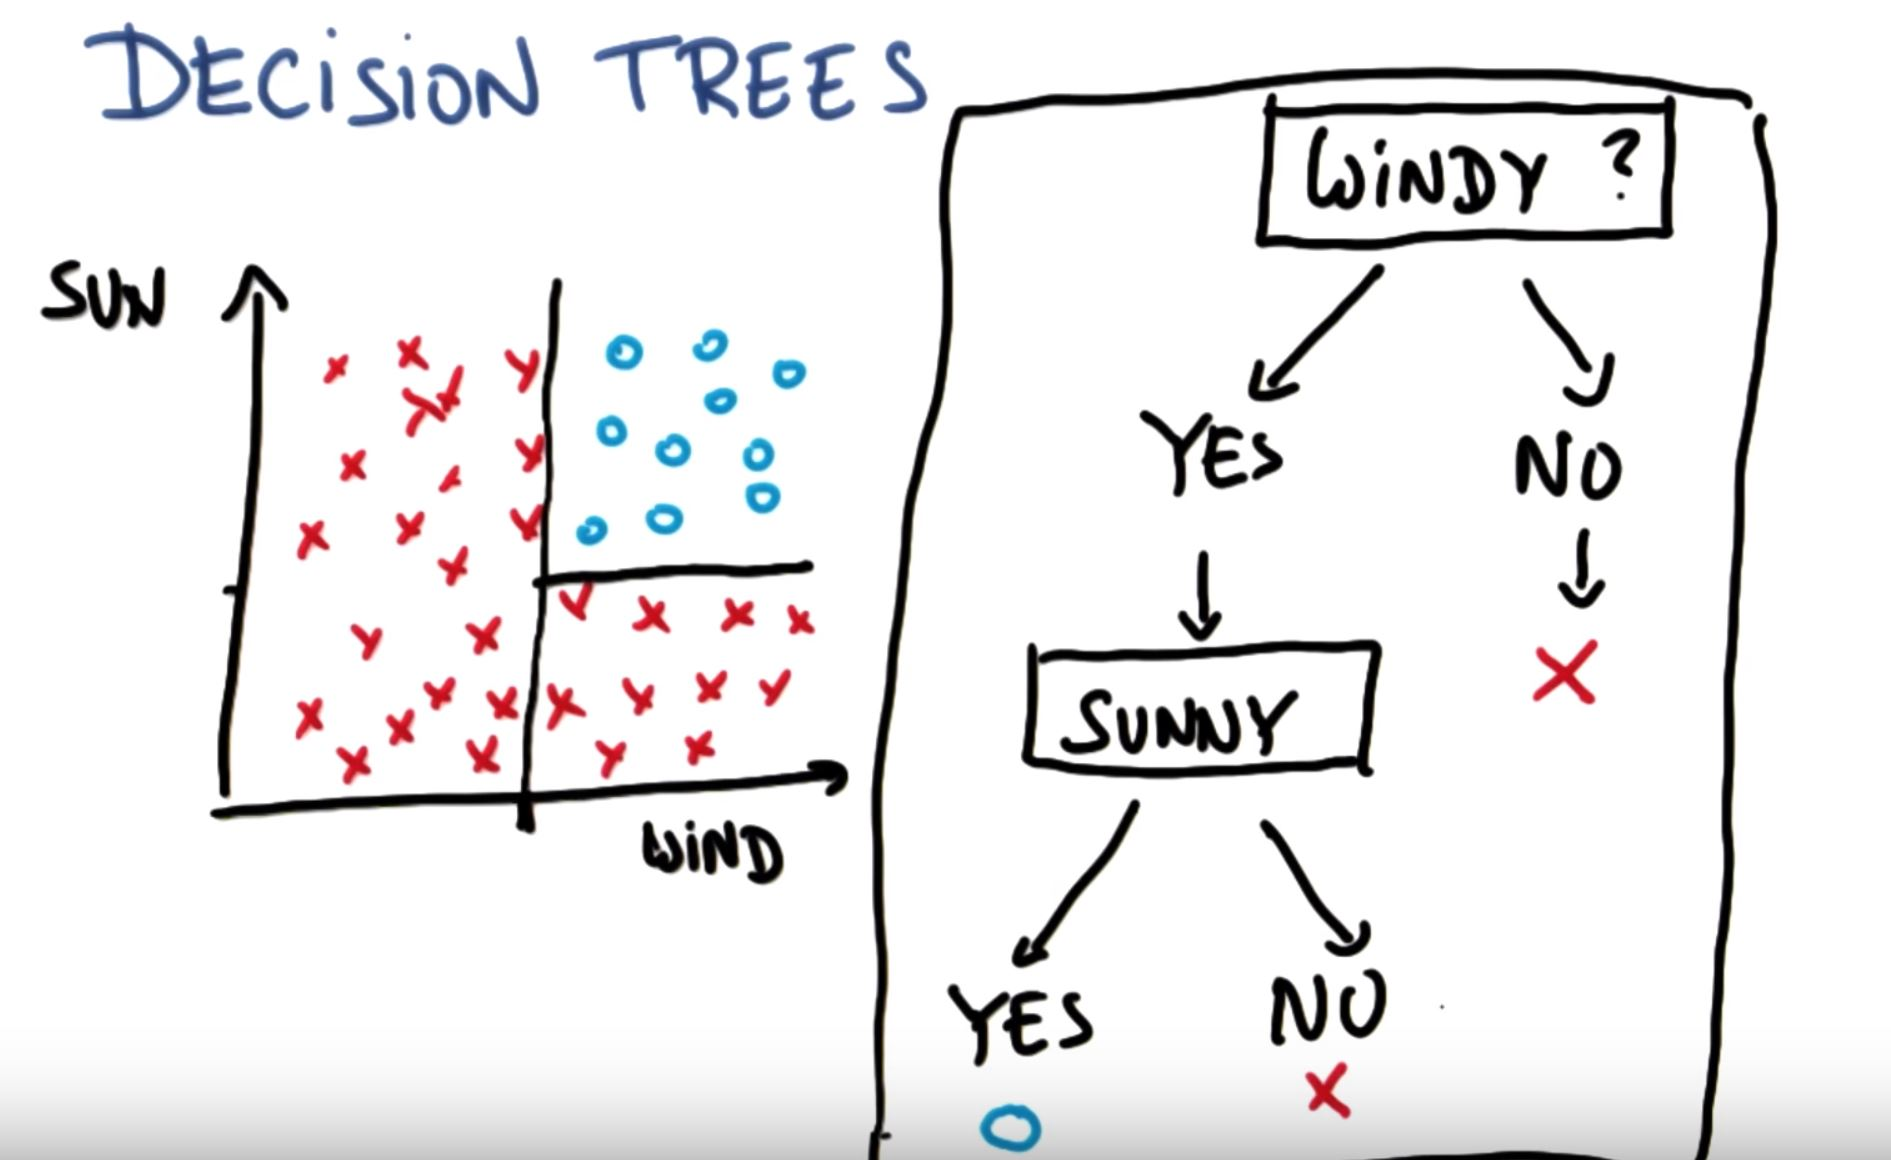
\includegraphics[width=0.6\textwidth]{pics/tree_linear_separator}
	\caption{Tree separator} 
	\label{tree_linear_separator}
\end{figure}
%         --------------------------------------


To improve performance, we can use many trees with a random sample of features chosen as the split.
\begin{itemize}
	\item  A new random sample of features is chosen for \textit{every single tree at every single split}.
	\item For classification, m (\# random features) is typically chosen to be the square root of p (\# total features).
\end{itemize}

Random Forests vs. Trees \\
Suppose there is \textit{one very strong feature} in the data set. When using “bagged” trees, most of the trees will use that feature as the top split, resulting in an ensemble of similar trees that are \textit{highly correlated}. Averaging highly correlated quantities does not significantly reduce variance. By randomly leaving out candidate features from each split, \textbf{Random Forests "decorrelates" the tree}s, such that the averaging process can reduce the variance of the resulting model.

\begin{lstlisting}
# 1. read data
df = pd.read_csv('kyphosis.csv')

# 2. visualise 
sns.pairplot(df,hue='Kyphosis',palette='Set1')

# 3. Decision Tree & Random Forest
 # train
from sklearn.model_selection import train_test_split
X_train, X_test, y_train, y_test = 
  train_test_split(df.drop('Kyphosis',axis=1),
   df['Kyphosis'], test_size=0.30)
  
  # build Decision Tree
from sklearn.tree import DecisionTreeClassifier
dtree = DecisionTreeClassifier()
dtree.fit(X_train,y_train)
predictions = dtree.predict(X_test)

 # build Random Forest (NB: .tree vs. .ensemble)
from sklearn.ensemble import RandomForestClassifier
rfc = RandomForestClassifier(n_estimators=100)
rfc.fit(X_train, y_train)
rfc_pred = rfc.predict(X_test)

 # evaluate
from sklearn.metrics import classification_report,confusion_matrix
print(confusion_matrix(y_test,predictions)) # for tree
print(confusion_matrix(y_test,rfc_pred))  # for rdm forest
# and same for classification_report
\end{lstlisting}

To reduce potential overfit, I can increase the min\_samples\_split (one param in DecisionTreeClassifier) from default of 2 (won't split samples lower than 2) to something bigger, e.g. 50.

%%%%%%%%%%%%%%%%%%%%%%%%%%%%%%%%%%%%%%%%%%%%%%%%%%%%%%
\subsection{Neural Network}

\subsubsection*{Perceptron}
Cartoonish view of human neurons.

Perceptron (see fig. \ref{perceptron} for a graphic definition) always returns half-plane (e.g. immagine 2 inputs $X$ with equal weights $1/2$ and a threshold of $3/4$, then the perceptron divides the plan in two by the line passing for (0,3/2) and (3/2,0): 1 above and zero below) - i.e. linear threshold units.

If the 'net-input' - which is a linear combinations of weights and inputs,  $w^T x$, also called 'activation' ??? - is above a threshold $\theta$ then the input belongs to one class, otherwise to the other (there are only two classes, a binary problem - NB: decision is a 'step function'). One can brings $theta$ on the left of the equation to simplify the problem ($w_0 = theta$, usually called the 'bias unit' - i.e. the new net-input is then compared to zero). In other words, the net input - $w^T x$ - is squashed into a binary output by the decision function, which is used to discriminate between two \textit{linearly-separable} classes.

'And', 'or' or 'not' are all expressible as perceptron untis - but 'Xor' is not

%          --------   FIGURE: percepton  -----------
\begin{figure}[htbp] 
	\centering
	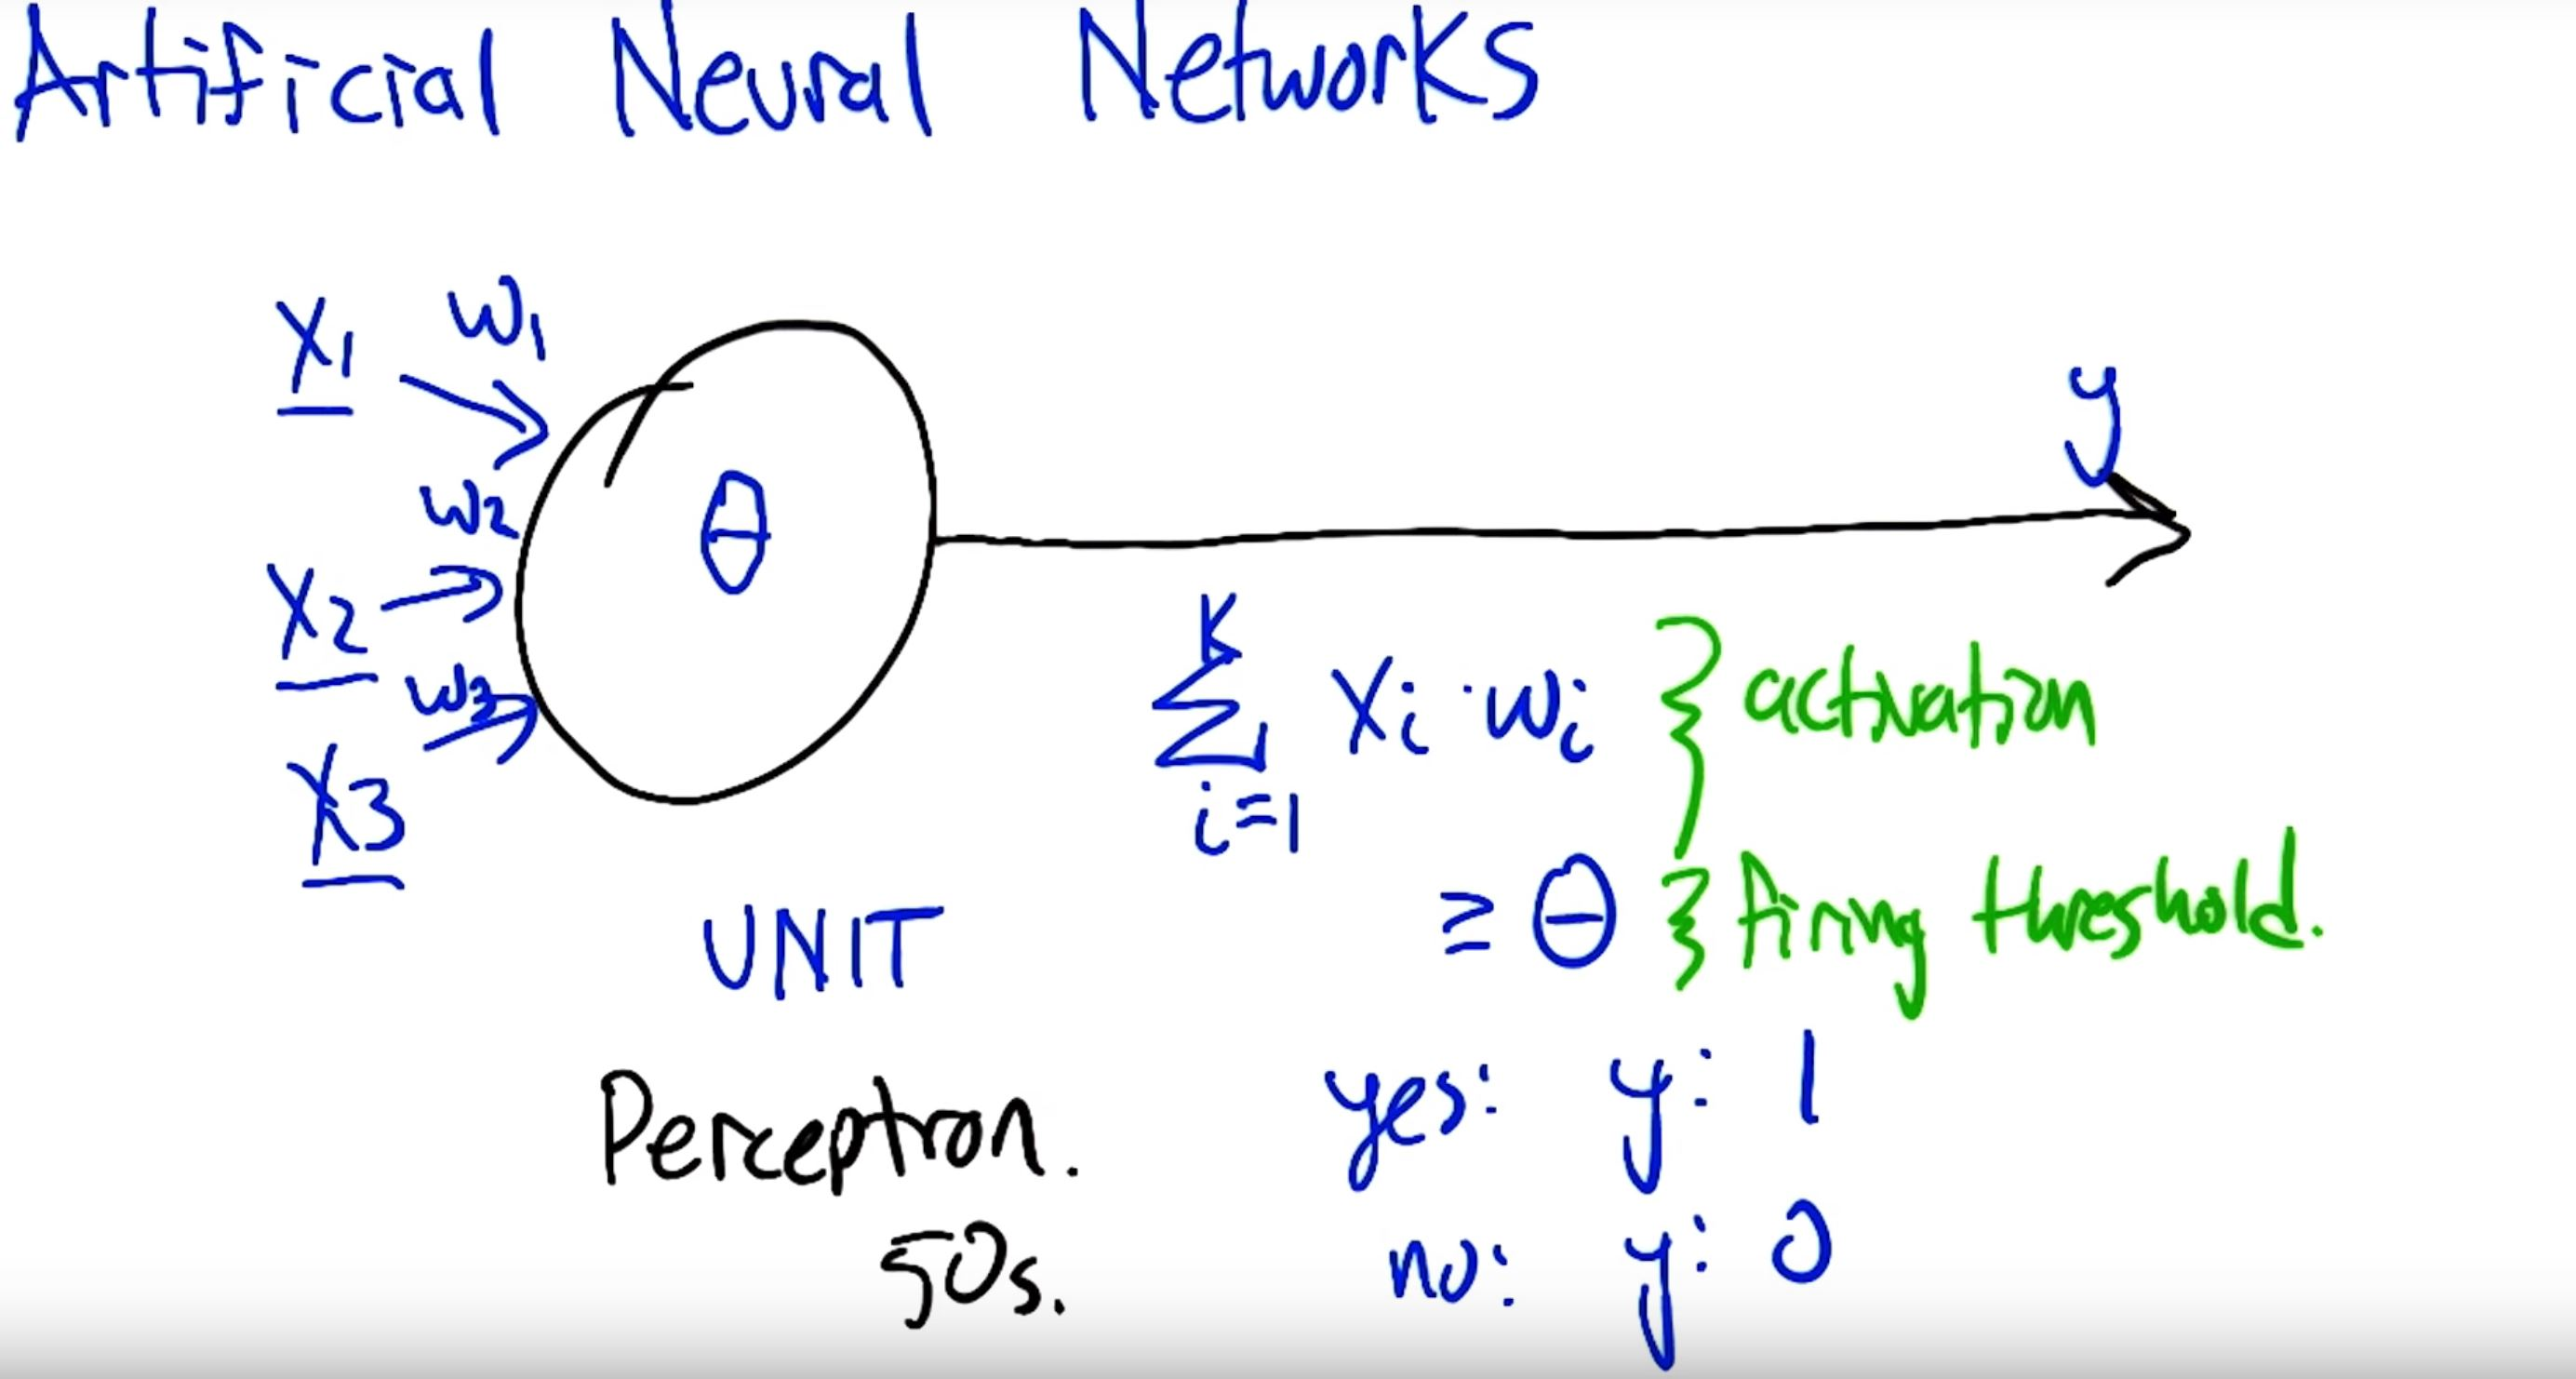
\includegraphics[width=0.7\textwidth]{pics/perceptron}
	\caption{Perceptron} 
	\label{perceptron}
\end{figure}
%         --------------------------------------
Rosenblatt's perceptron rules:
\begin{itemize}
	\item initialise weights to zero or small random numbers (reasons below);
	\item for each training sample/input: $x^{(i)}$:
	\begin{itemize}
		\item compute class output (using the step function)
		\item update weights: $w_j = w_j +  \underbrace{ \eta \, (y^{(i)} - predicted^{(i)}) x_j^{(i)}}_{\Delta w_j}$.
	\end{itemize}
\end{itemize}
where $\eta$ is the 'learning rate' in $(0., 1.]$.

The convergence of the perceptron is only guaranteed if the two classes are linearly separable and the learning rate is sufficiently small. Otherwise, it will never stop to update the weights. 
\begin{lstlisting}
# relevant part of a class
# X : {array-like}, shape = [n_samples, n_features]
# y : array-like, shape = [n_samples], Target values.

rgen = np.random.RandomState(self.random_state)
self.w_ = rgen.normal(loc=0.0, scale=0.01,
		   size = 1 + X.shape[1]) # 1 for 'bias unit'
self.errors_ = []
for _ in range(self.n_iter):  # limit iterations (e.g 50)
	errors = 0
	for xi, target in zip(X, y):	# loop through n_samples
		# xi is a vector of n_features
		net_input = np.dot(xi, self.w_[1:]) + self.w_[0]
		predict=np.where(net_input>=0.0, 1, -1) # unit step
		update = self.eta * (target - predict)
		self.w_[1:] += update * xi
		self.w_[0] += update
		errors += int(update != 0.0)
	self.errors_.append(errors)
return self
\end{lstlisting}
If all the weights were initialized to zero, the learning rate parameter $\eta$ would only affect the scale of the weight vector, not the direction (i.e. angle between vectors, via dot product, would be zero: 0. = np.arccos( v1.dot(v2) / (np.linalg.norm(v1) * np.linalg.norm(v2)) ).

\subsubsection*{Adaline}
ADAptive LInear NEuron (\textbf{Adaline}), by Widrow and Hoff. The key difference vs. the perceptron is that the weights are updated using a linear activation function instread that by a unit step fnct. In short, instead of comparing the target (true class) with the predicted class, Adaline compares the true class with the linear activation fnct value (which is here the identity fnct of the net input: $\phi(w^T x) = w^T x$, i.e. a real number). The advantageis that the linear activation fnct is \textit{differentiable} and convex. We can therefore use an objective fnct, in case of Adaline a SSE between true class and prediction that can be minimised:
\[ J(w) = \frac{1}{2} \sum_i (y^i - \phi(w^i \, x^i))
\] 
The term $1/2$ is used to make easier the gradient. We can update the weights by taking a step in the opposite direction of the gradient $\nabla J(w)$ multiplied by the learning rate, i.e. $\Delta w = -\eta \nabla J(w)$ (to compute the gradient we take the partial derivative of SSE with respect to each weight $w_j$):
\[ 
w_j = w_j +   \eta \, (y^{(i)} - \phi(w^i \, x^i)) x_j^{(i)}
\]
The rule seems identical, but $\phi$ is a real number and not an integer class, furthermore weights update is calculated on \textit{all} samples in the training set (instead than incrementally after each sample like in the perceptron), which is why this approach is called \textbf{batch gradient descent}.

\begin{lstlisting}
rgen = np.random.RandomState(self.random_state)
self.w_ = rgen.normal(loc=0.0, scale=0.01,
			size=1 + X.shape[1])
self.cost_ = []
for i in range(self.n_iter):
	net_input = net_input(X)
	output = activation(net_input)  # identity here
	errors = (y - output)
	self.w_[1:] += self.eta * X.T.dot(errors)  # gradient on all training set
	self.w_[0] += self.eta * errors.sum()  
	cost = (errors**2).sum() / 2.0
	self.cost_.append(cost)
return self

def net_input(self, X):
    return np.dot(X, self.w_[1:]) + self.w_[0]

def activation(self, X):
    return X

def predict(self, X):
    """Return class label after unit step"""
    return np.where(activation(net_input(X)) >= 0.0, 1, -1)
\end{lstlisting}
We have to choose $\eta$ and $self.n_iter$ -our \textbf{hyperparameters}- to minimise the $self.cost$ above.

Many learning algos, like gradient descent, benefits from features scaling: $x^{'}_j = 
(x_j - \mu_j) / \sigma_j$
\begin{lstlisting}
X_std = np.copy(X)
X_std[:,0] = (X[:,0] - X[:,0].mean()) / X[:,0].std()
\end{lstlisting}

A more computational efficient alternative to batch gradient descent (e.g. for millions of data points) is (online or) \textbf{stochatic gradient descent}, which is also useful for online learning.

\subsubsection*{More}
Neural network can represent booleans, continuous or arbitrary functions by just adding more \textbf{units} (more perceptrons, e.g. visually organised in a column) and (hidden) \textbf{layers} (number of columns) - so no restriction bias. To avoid overfit than limit numbers of units/layers and use cross-validation (same the trade-off bias vs. variance in other methods.)

In other words, neural networks are a bunch of perceptrons added together in parallel to form one layer and multiplying such layers separated by non-linear elements.

Backpropagation: get output given inputs by changing intermediate units and layers using gradient descent (one at the time).

Preference bias: algorithm's selection of one representation over another. Occam's razor.

Gradient descent: initial weights - generally small random values: random to avoid local minima by introducing variability, small for lower complexity because big weights may lead to overfitting)

%%%%%%%%%%%%%%%%%%%%%%%%%%%%%%%%%%%%%%%%%%%%%%%%%%%%%%
\subsection{Support Vector Machines}
Separate data using hyperplane (a line in 2-dim, a plane in 3-dim, ...), intuitively the best line is the one least committed to the data (not too close to one of the classes in our training data), or in other words, the one that maximises the distance between the nearest points of the classes and the line/hyperplane, that distance is called \textbf{margin} in SVM (the idea is that of robustness: we use the training data, but we don't trust them too much - so we keep equidistant).
%          --------   FIGURE: SVM  -----------
\begin{figure}[htbp] 
	\centering
	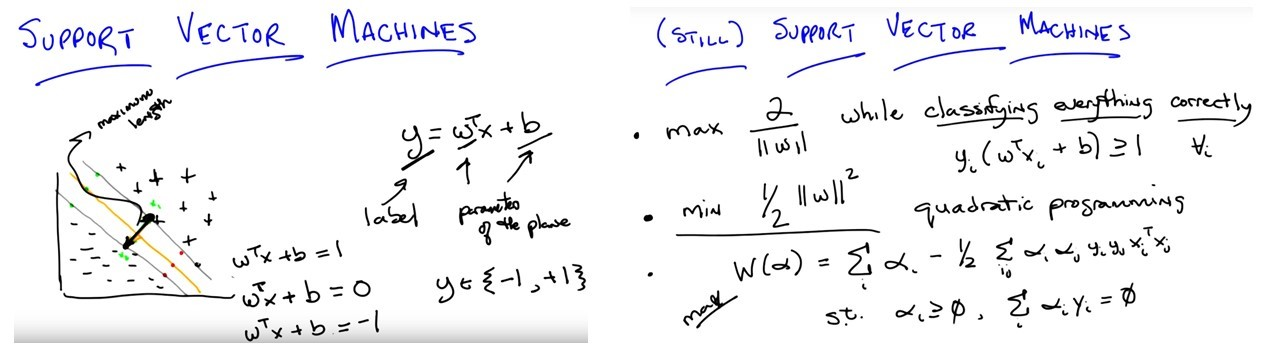
\includegraphics[width=1.\textwidth]{pics/SVM}
	\caption{SVM} 
	\label{SVM}
\end{figure}
%         --------------------------------------

In order to maximise such distance, we can subtract the two boundaries from one another (see left-hand side fig. \ref{SVM}) and be left with $w^T (x_1-x_2) = 2$, then divide by the norm of $w$. Hence we need to maximise $2 /||w|| $ subject to $y_i (w^T x_i + b) \geq 1 ;\forall i$ (note that we multiply by $y_i$ to avoid writing two inequalities for $(\dots)$ $\leq -1$ and $\geq 1$ ). 
An equivalent, but easier (quadratic: unique solution) problem is to minimise $1/2 \,||w||^2$ with same constraints - that again can transform into another quadratic problem with $alpha$ as new param(s) (see right-hand side fig. \ref{SVM}). We can then recover $w$ simply as $w=\sum_i \alpha_i y_i x_i$ and since most of alphas are zero, one only needs a few of $x_i$ matter (you can see intuitively in a plane that the $x_i$ closer to the separating line matter).

We can use the \textbf{kernel trick} (adding one or further dimensions) to separate classes linearly with an hyper-plan - see fig. \ref{kernel_trick}, the kernel is the transformation we are applying to the dot product ($x_i x_j$) in fig \ref{kernel_trick}. Besides $k = (x^T y)^2$ in the fig (called '\textit{linear}'), there are many other possible transformations like the gaussian-looking '\textit{rbf}' $k(x,y)= \exp(-\gamma ||x-y||^2)$) or the \textit{sigmoid} $\tanh(\alpha x^y y + \theta)$. A Kernel must satisfy the \underline{Mercer condition}, i.e. intuitively it must act as a distance/inner product\footnote{The kernel trick avoids the \textit{explicit} mapping that is needed to get \textit{linear} learning algorithms to learn a \textit{nonlinear} function or decision boundary. For all x and y in the input space, certain functions $k(x,y)$ can be expressed as an inner product in another space - the $k$ map is called \textit{kernel} (the word 'kernel' is generally used in mathematics to denote a weighting function for a weighted sum or integral).}. 

%          --------   FIGURE: Kernel trick  -----------
\begin{figure}[htbp] 
	\centering
	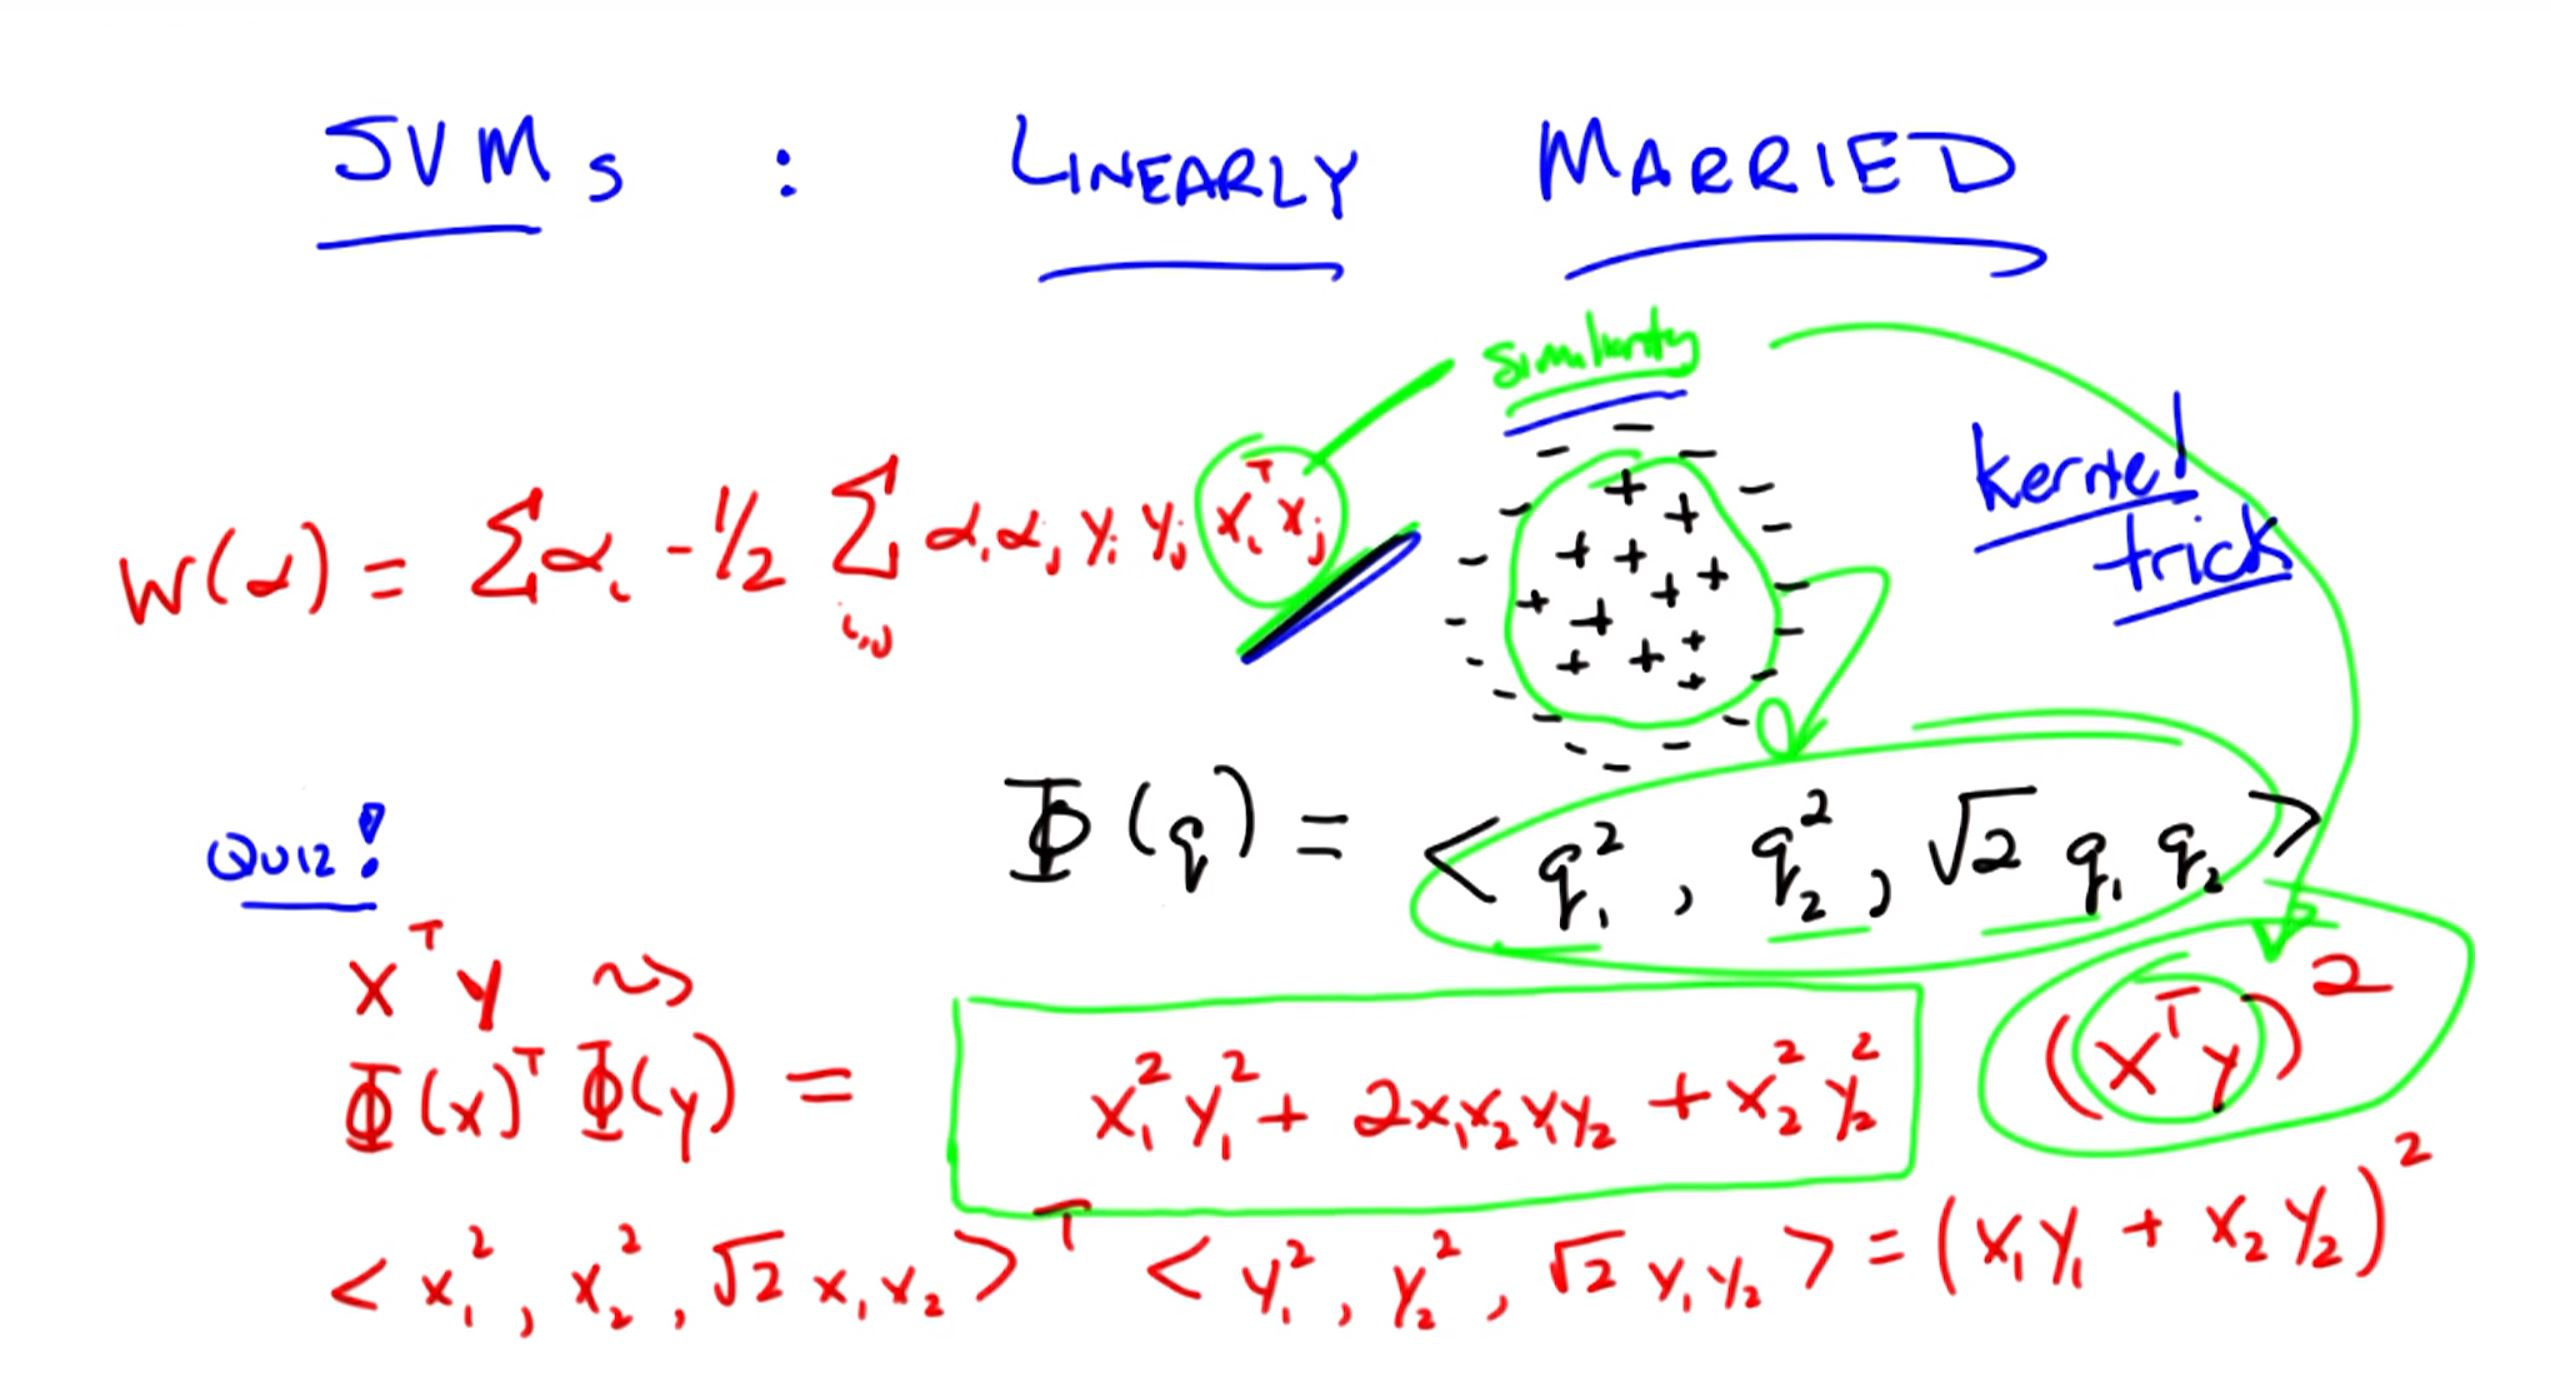
\includegraphics[width=.9\textwidth]{pics/kernel_trick}
	\caption{Kernel trick (SVM)} 
	\label{kernel_trick}
\end{figure}
%         --------------------------------------


Coding example using a built-in dataset:
\begin{lstlisting}
# 1. get data
from sklearn.datasets import load_breast_cancer
cancer = load_breast_cancer()

cancer.keys() # data shown in dict keys
# -> dict_keys(['DESCR', 'target', 'data', 'target_names', 'feature_names'])
print(cancer['DESCR'])  # long description
 
 #set-up df of the features and target
df_feat = pd.DataFrame(cancer['data'], 
					columns=cancer['feature_names'])
df_target = pd.DataFrame(cancer['target'], columns=['Cancer'])

# 2. do some explanatory data analysis
# e.g. sns.pairplot with hue = target

# 3. S V Classifier
 # train split
from sklearn.model_selection import train_test_split
X_train, X_test, y_train, y_test = 
	train_test_split(df_feat, df_target, 
	test_size=0.30, random_state=101)
	
  # build 'naive' SVC: WRONG WAY
from sklearn.svm import SVC
model = SVC()
model.fit(X_train,y_train)
predictions = model.predict(X_test)

 # evaluate
from sklearn.metrics import classification_report,confusion_matrix
print(confusion_matrix(y_test,predictions))
print(classification_report(y_test,predictions))
# all classficed into a single class... we need GridSearch

 
 # build SVC properly: use GridSearch (meta-estimator)
from sklearn.model_selection import GridSearchCV
param_grid = {'C': [0.1,1, 10, 100, 1000], # is C not gamma? CHECK!!!
	'gamma': [1,0.1,0.01,0.001,0.0001], 'kernel': ['rbf']}  
grid = GridSearchCV(SVC(),param_grid,refit=True,verbose=3)	
# rbf: this is actually default, get verbose>0 to see some output
grid.fit(X_train,y_train)  # May take awhile!
grid.best_params_    # show best params
grid.best_estimator_ # show best estimator
grid_predictions = grid.predict(X_test)

 # evaluate (will be much better than naive one above)
print(confusion_matrix(y_test,grid_predictions))
print(classification_report(y_test,grid_predictions))
\end{lstlisting}
Besides the \textbf{Kernel} (linear, poly, rbf which is the default, sigmoid, or even a custom one), there are two more params: (i) \textbf{C}, the penalty parameter of the error term (it controls the tradoff between \textit{smooth} decision boundary and classifying training points \textit{correctly}: the lower the smoother the boundary, the higher the more correct) and (ii) \textbf{gamma} (coefficient for ‘rbf’, ‘poly’ and ‘sigmoid’ - hence no effect on the 'linear' kernel; it can be seen as the inverse of the radius of influence of samples selected by the model as support vectors; too large and it will overfit, too small and it will be too constrained).


%%%%%%%%%%%%%%%%%%%%%%%%%%%%%%%%%%%%%%%%%%%%%%%%%%%%%%
\subsection{Ensemble}
You get some simple rules and combine them to get a complex rule (learn over a subset of data that generates a rule, repeat, and combine all).

%
\subsubsection{Bagging}
\textbf{Bagging or Bootstrapping aggregation}: combine simple rule(s) (e.g. 3rd order polynomial) on \textbf{random subsets} of the training data and average the result. 

Bagging is the simplest ensemble learning we can think of: 
\begin{itemize}
	\item Simplest way to choose data: select uniformly randomly subsets.
	\item Simplest combination: simple average.
\end{itemize}

Such an ensemble learning tends to perform \underline{better on the test/validation} datasets (lower variance) than more complex models (e.g. a 4rd order polynomial fitted on all training dat, which obviously fits better: lower bias).

%
\subsubsection{Boosting}
Let's improve on Bagging by (i) focusing on the \textbf{'hardest'} examples and using (ii) \textbf{weighted} mean.0.5

Introducing a new error defition (rather than simple mistmatch) as probability - given a distribution - that my Hp disagrees with the truth concept on some instances $x$ : $Pr_{distr}[Hp(x) \neq c(x)]$. 

Concept of \textbf{weak learner}: no matter the distribution of the data, it gets lower errors than chance (e.g. <0.5): prob above is $ \ldots \leq 0.5 - \epsilon$.

%          --------   FIGURE: Boosting  -----------
\begin{figure}[htbp] 
	\centering
	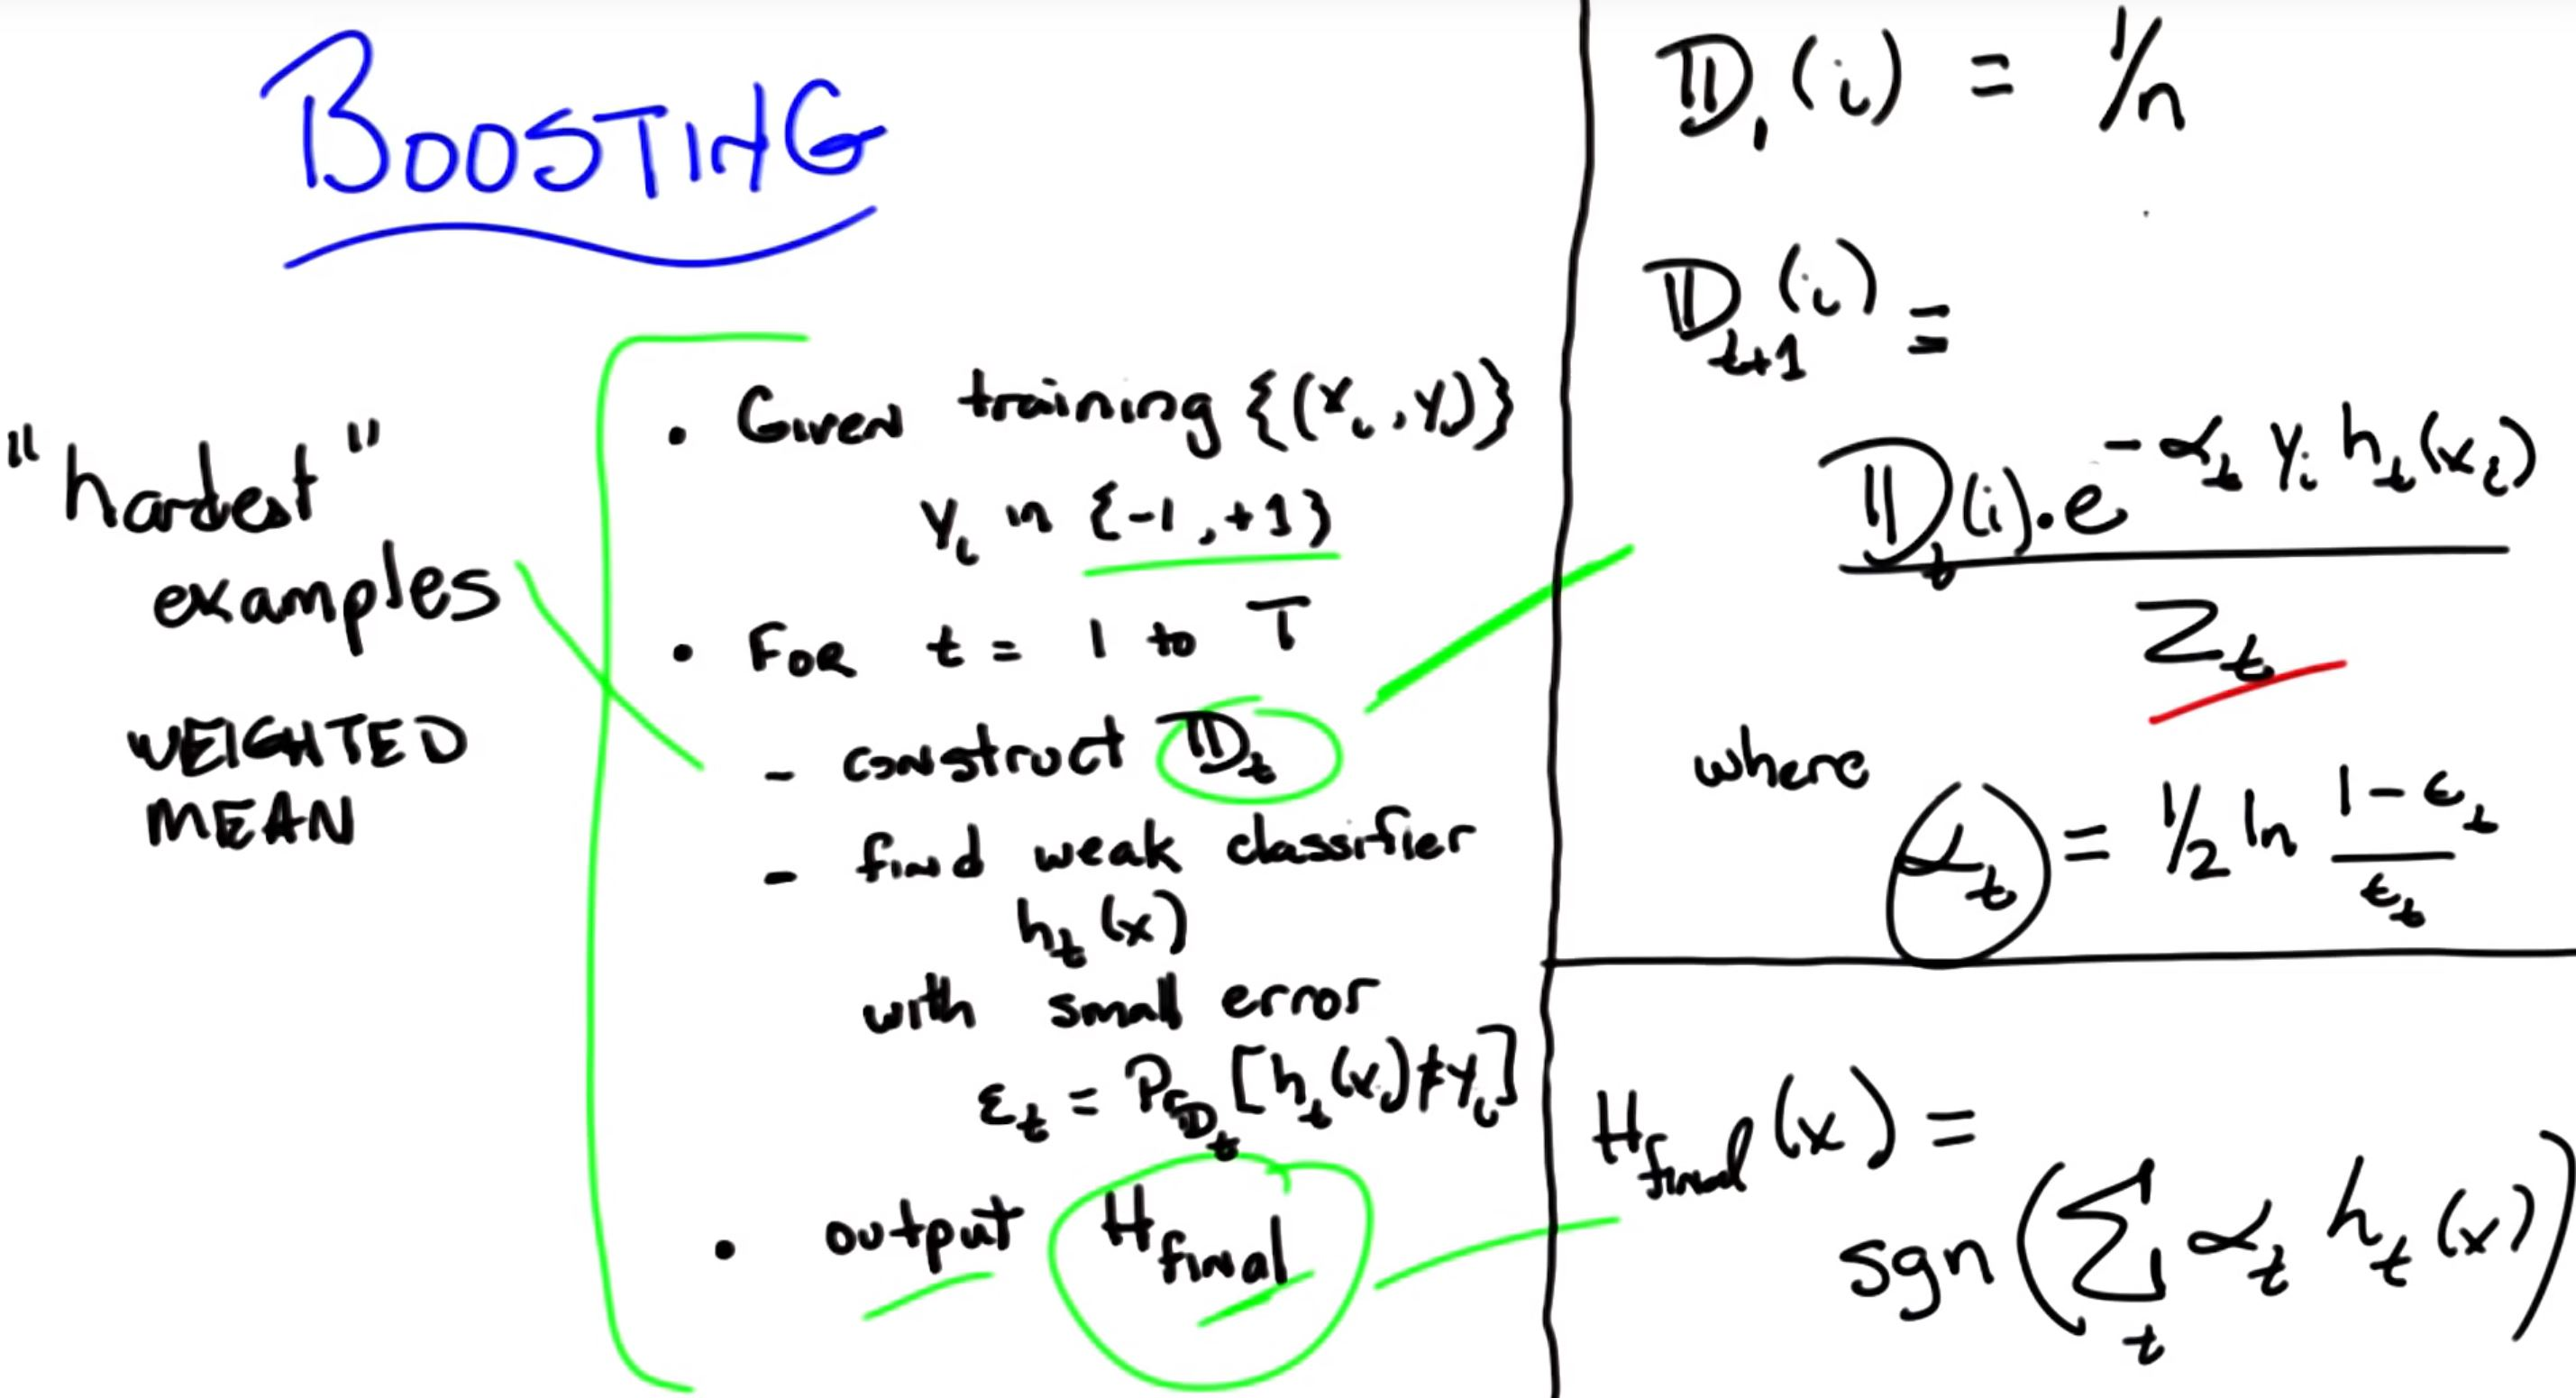
\includegraphics[width=.9\textwidth]{pics/boosting_1}
	\caption{Boosting algorithm} 
	\label{boosting_1}
\end{figure}
%         --------------------------------------
In fig. \ref{boosting_1}: note that if $y_i$ and $h_t(x_i)$ agrees (i.e. both $+1$ or $-1$), considering that $alpha$ is positive, the single $D_{t+1}(i)$ decreases (but the whole $D_{t+1}$ depends on other $x_i$). The final $H_{final}$ is a weighted function of the $h$ (if you divide by $sum_i \alpha_i$, that becomes a weighted average and answers remains the same): as we keep adding more and more learners, the error may not decrease much - but our confidence increases (more certain about harder example - we increase the margin), which helps avoiding overfitting. Boosting is agnoistic to the learner, as long as a 'weak' learner (better than 50%).

Boosting may overfit if (i) the underlying learner overfits from the start (e.g. ANN with many layers) any looping does not make it better, (ii) 'pink noise' (uniform noise). 


%%%%%%%%%%%%%%%%%%%%%%%%%%%%%%%%%%%%%%%%%%%%%%%%%%%%%%
\subsection{K Means Clustering}
K Means Clustering is an \textbf{unsupervised} learning algorithm that will attempt to group similar elements (PCA instead is a factor based rather than clustering algo). Used for market segmentation, cluster customers based on features, identify similar groups, ...

The K Means Algorithm consists of the following steps:
\begin{itemize}
	\item choose a number of clusters “K” (more details later),
	\item randomly assign each point to a cluster
	\item until clusters stop changing, repeat the following loop: (i) for each cluster, compute the cluster centroid by taking the mean vector of points in the cluster and (ii) assign each data point to the cluster for which the centroid is the closest.
\end{itemize}
%          --------   FIGURE: k_means_algo_loop  -----------
\begin{figure}[htbp] 
	\centering
	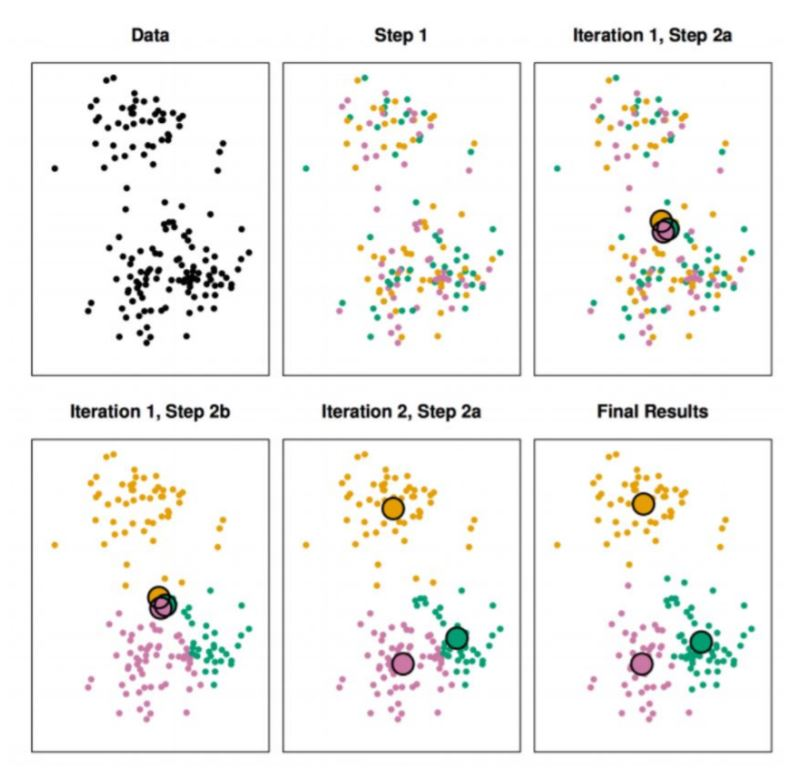
\includegraphics[width=0.6\textwidth]{pics/k_means_algo_loop}
	\caption{K Means algorithm} 
	% \label{k_means_algo}
\end{figure}
%         --------------------------------------

There is no easy answer on how to choose the best K. One way is the  elbow method:
\begin{itemize}
	\item compute, for some K values (e.g. 2, 4, 6, 8, etc.), the sum of squared error (SSE) between each cluster member and its centroid,
	\item if you plot K vs. SSE you will see that the error decreases as k gets larger, the idea is to choose he K at which SSE decreases abruptly (this produce an elbow effect n the graph - see following fig) 
\end{itemize} 
%          --------   FIGURE: elbow  -----------
\begin{figure}[htbp] 
	\centering
	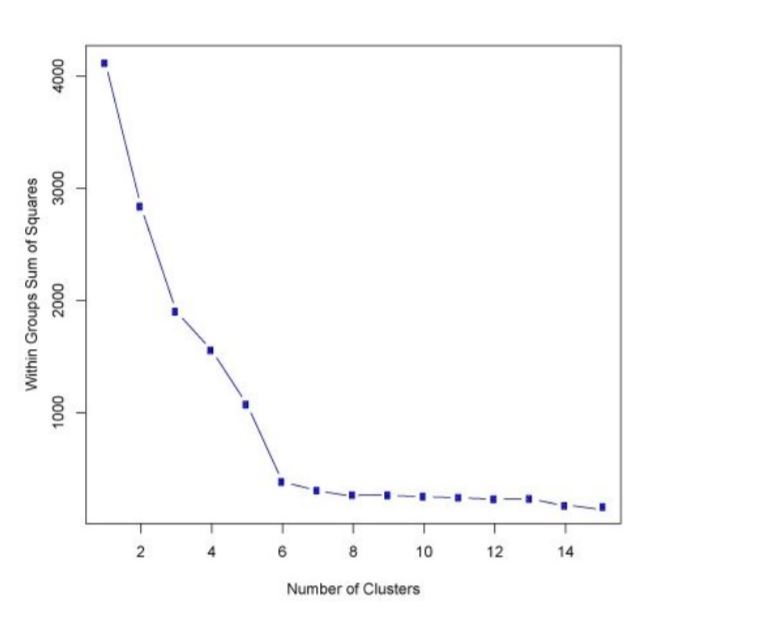
\includegraphics[width=0.6\textwidth]{pics/elbow}
	\caption{Choosing a K value: elbow method} 
	% \label{elbow}
\end{figure}
%         --------------------------------------

\begin{lstlisting}
# 1. get/create data
from sklearn.datasets import make_blobs # arrays
# Create Data
data = make_blobs(n_samples=200, n_features=2, 
centers=4, cluster_std=1.8,random_state=101)

# 2. do some explanatory data analysis
plt.scatter(data[0][:,0],data[0][:,1],c=data[1],cmap='rainbow')
# 'c=' is the color


# 3. K Means Clustering
 # create the cluster (NB: no train_test) 
from sklearn.cluster import KMeans
kmeans = KMeans(n_clusters=4) # choose the no. of clusters
kmeans.fit(data[0])

 # output
kmeans.cluster_centers_  # coordinates for K's
kmeans.labels_  # the labels, see charts below

 # visual output: K mean vs. original (NB: only in our example 
 # since we've the labels - not possible since unsupervised)
f, (ax1, ax2) = plt.subplots(1, 2, sharey=True,figsize=(10,6))
ax1.set_title('K Means')  # the chart with the label (NB: 'c=')
ax1.scatter(data[0][:,0],data[0][:,1],c=kmeans.labels_,cmap='rainbow')
ax2.set_title("Original")
ax2.scatter(data[0][:,0],data[0][:,1],c=data[1],cmap='rainbow')
\end{lstlisting}

%%%%%%%%%%%%%%%%%%%%%%%%%%%%%%%%%%%%%%%%%%%%%%%%%%%%%%
\subsection{Principal Component Analysis}
Principal Component Analysis (PCA) is an \textbf{unsupervised} learning algorithm (like K-Means Clustering).

In short, PCA is a transformation of data in attempts to find out what features explain the most variance in the data.

It is difficult to visualize high dimensional data, we can use PCA to find the first two principal components, and visualize the data in this new, two-dimensional space, with a single scatter-plot. Before we do this though, we'll need to scale our data so that each feature has a single unit variance (see scaler() below, in 2. PCA Visualition, or K-Nearest Neighbours \ref{K_Nearest_Neighbours}).

\begin{lstlisting}
# 1. Get the data
from sklearn.datasets import load_breast_cancer
cancer = load_breast_cancer()
cancer.keys()  # dict_keys(['DESCR', 'data', 
			   # 'feature_names', 'target_names', 'target'])
print(cancer['DESCR'])
df = pd.DataFrame(cancer['data'],columns=cancer['feature_names'])

# 2. PCA Visuation (but first scale data)
from sklearn.preprocessing import StandardScaler
scaler = StandardScaler() 
scaler.fit(df)
scaled_data = scaler.transform(df)

from sklearn.decomposition import PCA  # NB: .[family]
pca = PCA(n_components=2)  # instantiate
pca.fit(scaled_data)  # find the components (fittinh)
x_pca = pca.transform(scaled_data)  # rotation and dim reduction

scaled_data.shape  # e.g. (569, 30) vs. below
x_pca.shape  # (569, 2)  

plt.figure(figsize=(8,6))
plt.scatter(x_pca[:,0],x_pca[:,1],c=cancer['target'],cmap='plasma')
plt.xlabel('First principal component')
plt.ylabel('Second Principal Component')

# components stored as attributes
pca.components_

# each row in the matrix array above is a princ. component
# and each column related to orginal features
# We can visualize such relationship with a heatmap:
df_comp = pd.DataFrame(pca.components_,columns=cancer['feature_names'])
plt.figure(figsize=(12,6))
sns.heatmap(df_comp,cmap='plasma')
# color bar represents corr(feature, principal)
\end{lstlisting}

Unfortunately, with this great power of dimensionality reduction, comes the cost of being able to easily understand what these components represent. The components correspond to combinations of the original features, the components themselves are stored as an attribute of the fitted PCA object.

%%%%%%%%%%%%%%%%%%%%%%%%%%%%%%%%%%%%%%%%%%%%%%%%%%%%%%
\subsection{Recommender systems}
To be completed


%%%%%%%%%%%%%%%%%%%%%%%%%%%%%%%%%%%%%%%%%%%%%%%%%%%%%%
\subsection{Natural Language Processing (NLTK)}
To be completed

%%%%%%%%%%%%%%%%%%%%%%%%%%%%%%%%%%%%%%%%%%%%%%%%%%%%%%
\subsection{Big Data (Spark)}
To be completed

%%%%%%%%%%%%%%%%%%%%%%%%%%%%%%%%%%%%%%%%%%%%%%%%%%%%%%
\subsection{Deep Learning (Tensorflow)}
To be completed

%%%%%%%%%%%%%%%%%%%%%%%%%%%%%%%%%%%%%%%%%%%%%%%%%%%%%%%%%%%%%%%%%%%%%%%%%%%
%%					APPENDIX
\clearpage
\appendix
%Note that this is quite similar to Equation~\eqref{eq:eqA} in Appendix~\ref{sec:app1}.
%%%%%%%%%%%%%%%%%%%%%%%%%%%%%%%%%%%%%%%%%%%%%%%%%%%%%%%%%%%%%%%%%%%%%%%%%%%
%% 					Appendix 1
\section{From scratch}\label{sec:app1}
Some interesting, but not directly related topics are reported here.


\begin{lstlisting}
from sklearn.metrics import make_scorer
from sklearn.tree import DecisionTreeRegressor
from sklearn.model_selection import GridSearchCV

def fit_model(X, y):
   """ Performs grid search over the 'max_depth' parameter for a 
   decision tree regressor trained on the input data [X, y]. """

   # Create cross-validation sets from the training data
   cv_sets = ShuffleSplit(n_splits = 10, test_size = 0.20, random_state = 0)

   # Create a decision tree regressor object
   regressor = DecisionTreeRegressor()

   # Create a dictionary for the parameter 'max_depth' with a range from 1 to 10
   params = {'max_depth':[i for i in range(1,11)]}

   # Transform 'performance_metric' into a scoring function using 'make_scorer' 
   scoring_fnc = make_scorer(performance_metric)

   # Create the grid search cv object --> GridSearchCV()
   # (estimator, param_grid, scoring, cv) 
   grid = GridSearchCV(regressor, param_grid=params, scoring=scoring_fnc, cv=cv_sets)

   # Fit the grid search object to the data to compute the optimal model
   grid = grid.fit(X, y)

   # Return the optimal model after fitting the data
   return grid.best_estimator_
\end{lstlisting}


%          --------   Bayesain quiz  -----------
\begin{figure}[htbp] 
	\centering
	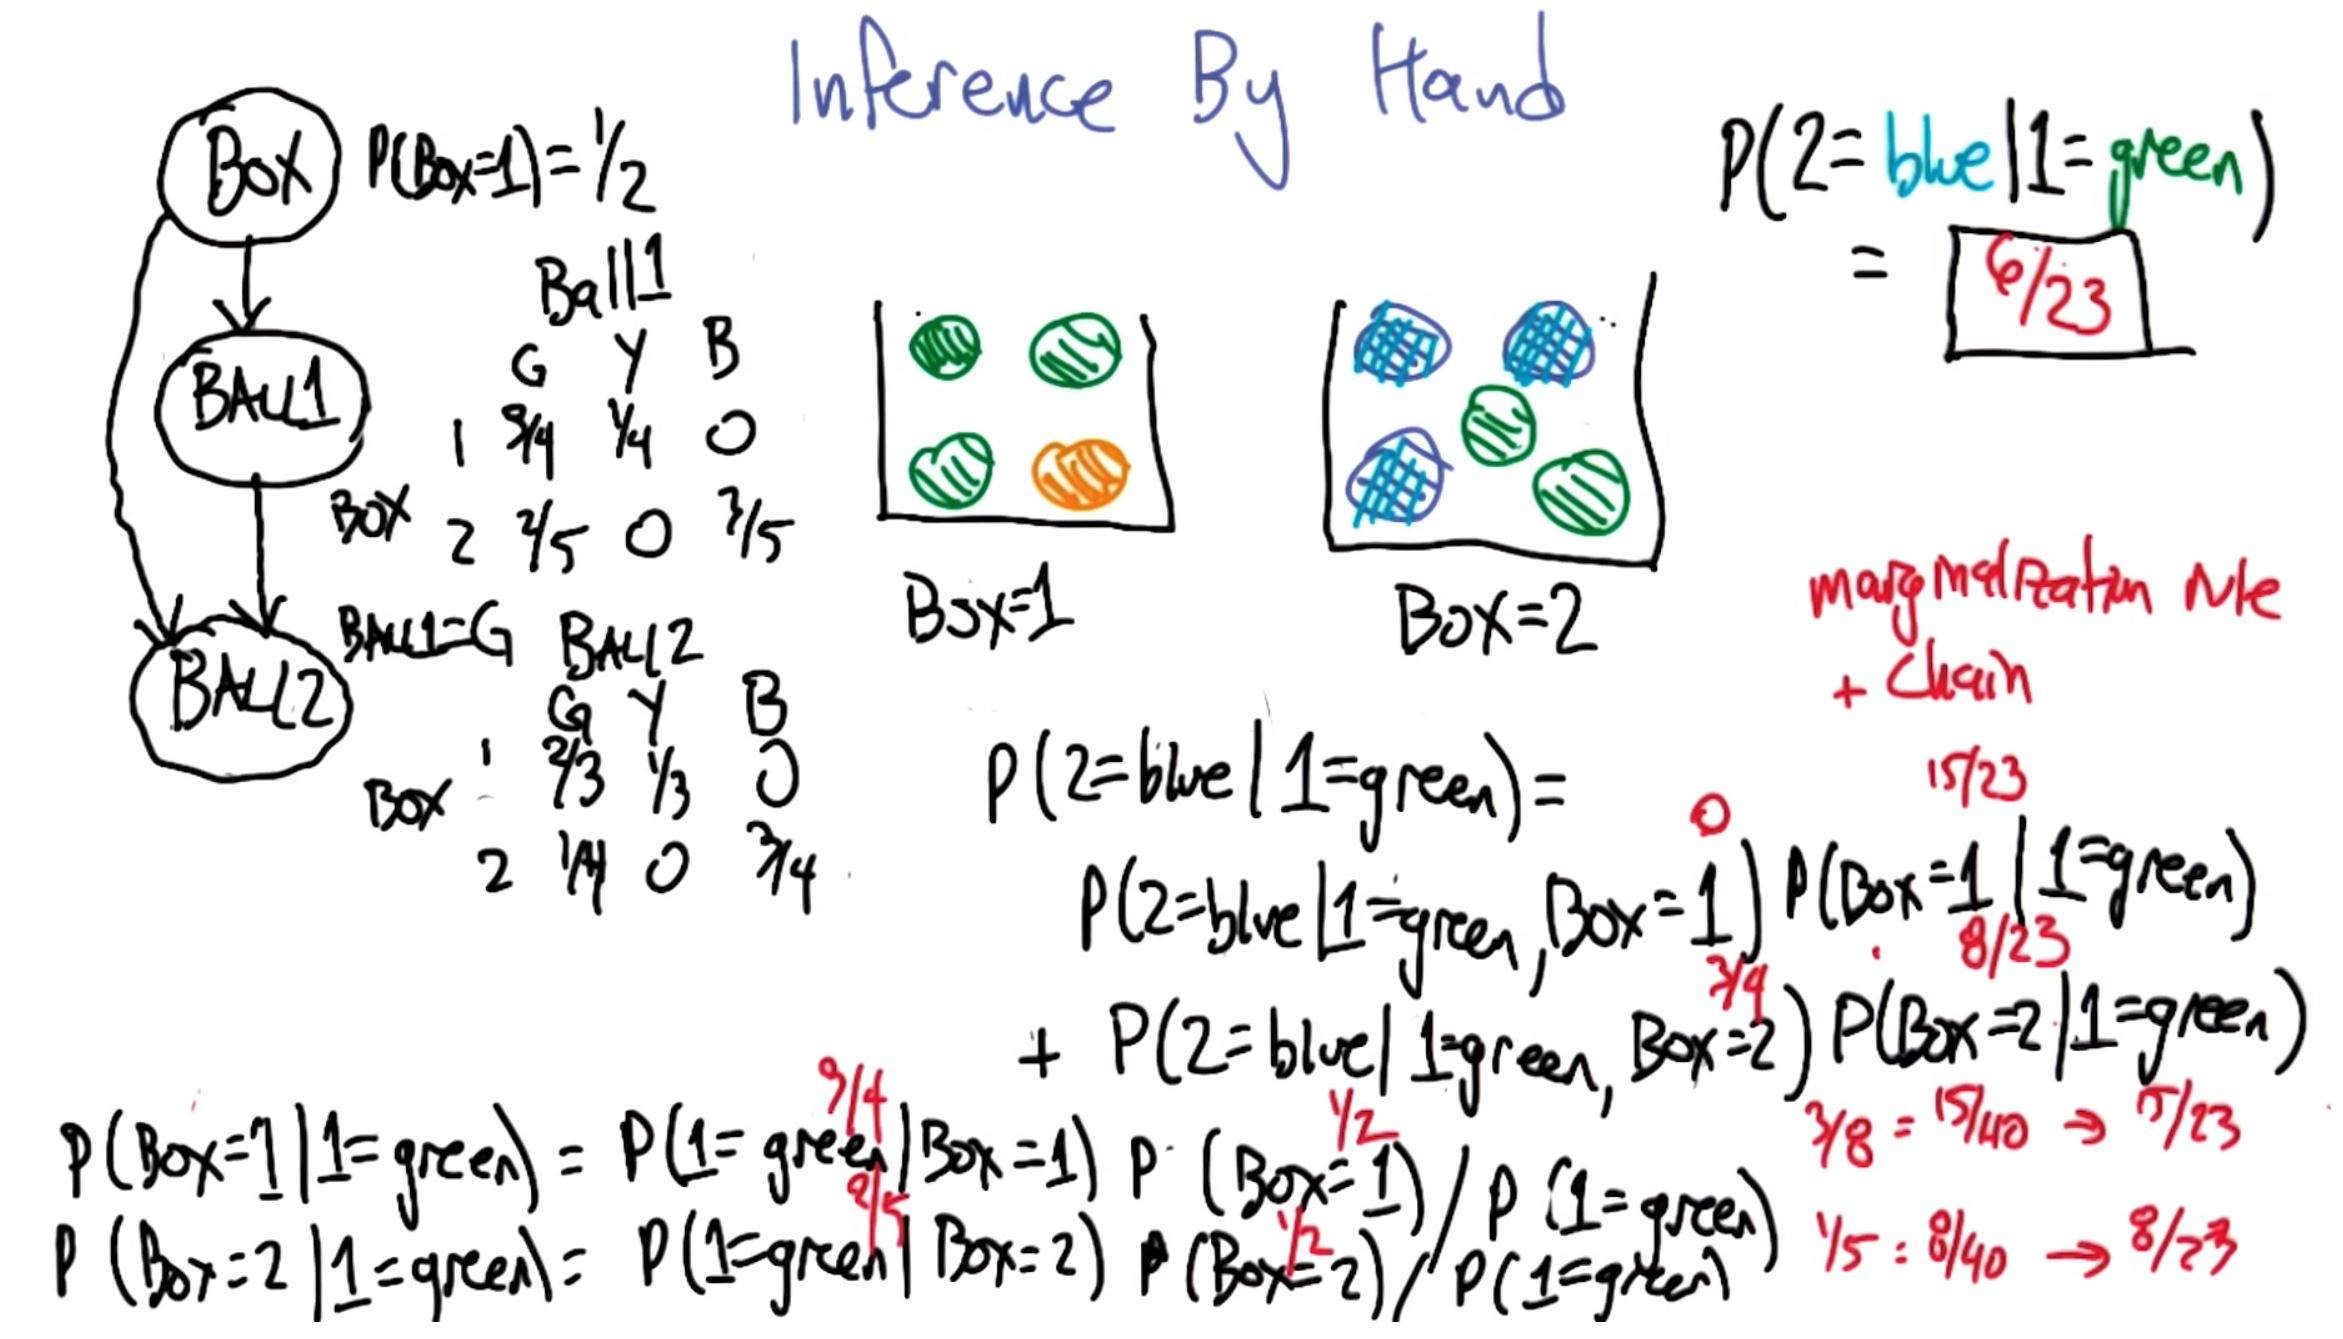
\includegraphics[width=0.9\textwidth]{pics/quiz_bayes}
	\caption{Bayes quiz} 
	\label{bayes_quiz}
\end{figure}
%         --------------------------------------

\clearpage

%%%%%%%%%%%%%%%%%%%%%%%%%%%%%%%%%%%%%%%%%%%%%%%%%
% Bibliography.
%%%%%%%%%%%%%%%%%%%%%%%%%%%%%%%%%%%%%%%%%%%%%%%%%

%% adds the bibliography to the table of contents: usato per la tesi
%  \addcontentsline{toc}{chapter} 
%  {\protect\numberline{Bibliography\hspace{-96pt}}} 

%% uncomment almeno le due seguenti
%  \bibliographystyle{jfe} % stile della biblio
%  \bibliography{allrefs} % nome del file dove raccogliere le bibliografie

\clearpage

% \ 
% \vfill
% \begin{figure}[!htb]
%  \centerline{\includegraphics[width=7in]{pics/Figure1}}
%  \caption{Structure of model. Capital can be invested in a bank sector and an equity sector. An intermediary has the expertise to reallocate capital between the sectors andto monitor bank capital against bank crashes.} \label{fig:0}
%  \end{figure}
% \vfill
% \ 
	
\end{document}




% --- esempio di come si include la bibliografia ---
% Among the interesting books and papers I have read in the course of this work is 
% Halzen and Martin's {\it Quarks and Leptons}\,\cite{Halzen:1984mc}, and the paper {\it Can
% one probe the structure of the pomeron?} by Ellis and
% Ross,\cite{Ellis:1996cg}.

% or for the "journal of finance" kind of style, we can also have the following options: \citeyear{fama/french:88-jpe} produces (1988b), and \citename{fama/french:88-jpe} produces Fama and French. 

% HYPERREF
% \url{http://www.wikibooks.org}
%  \href{http://www.wikibooks.org}{Wikibooks home}
% Both point at the same page, but in the first case the URL will be shown, while in the second case the URL will be hidden. Note that, if you print your document, the link stored using \href will not be shown anywhere in the document.


% IMPORTANT:
% --- When processing the file, you need to do: LATEX filename, BIBTEX filename, LATEX filename, LATEX filename ---